\documentclass[11pt]{amsart}
\usepackage{amsmath,amssymb,amsthm,mathtools}
\usepackage[margin=1.15in]{geometry}
\usepackage[expansion=false]{microtype}
\usepackage{enumitem}
\usepackage{booktabs}
\usepackage{tikz}
\usetikzlibrary{calc}
\usepackage[colorlinks=true,linkcolor=blue!45!black,citecolor=blue!45!black,urlcolor=blue!45!black]{hyperref}

\newtheorem{theorem}{Theorem}[section]
\newtheorem{proposition}[theorem]{Proposition}
\newtheorem{lemma}[theorem]{Lemma}
\newtheorem{corollary}[theorem]{Corollary}
\theoremstyle{definition}
\newtheorem{example}[theorem]{Example}
\theoremstyle{remark}
\newtheorem{remark}[theorem]{Remark}

\newcommand{\R}{\mathbb{R}}
\newcommand{\E}{\mathbb{E}}
\newcommand{\cT}{\mathcal{T}}
\newcommand{\PL}{\mathrm{PL}}
\newcommand{\st}{\operatorname{st}}
\newcommand{\Tr}{\operatorname{Tr}}
\newcommand{\Reff}{R_{\mathrm{eff}}}
\newcommand{\Ot}{\widetilde{O}}
\newcommand{\lo}{\preccurlyeq}
\newcommand{\eps}{\varepsilon}
\DeclareMathOperator{\diam}{diam}
\DeclareMathOperator{\exc}{exc}

\title[Duffin's networks, hyperbolic volume, Laplacian solvers]{Duffin's resistor networks, the volume of ideal polyhedra,\\ and nearly-linear-time Laplacian solvers}
\date{18 September 2026}

\raggedbottom
\begin{document}

\begin{abstract}
Discretizing the Dirichlet problem on a triangulated planar domain by piecewise-linear functions
produces a resistor network whose conductances are given by the cotangent formula (MacNeal 1949, Duffin 1959).
An edge has nonnegative conductance exactly when it is locally Delaunay, and the stiffness matrix is then a graph Laplacian.
The same matrix is, up to the factor $-2$, the Hessian of the hyperbolic volume of the ideal polyhedron over the triangulation, in the coordinates in which Rivin's variational principle for polyhedra with prescribed dihedral angles is naturally written.
Newton's method for that principle is therefore a sequence of Dirichlet problems on Duffin's network, with conductances that are positive throughout because the dihedral angles are data.
This note collects the precise statements: the network and its maximum principle, Rippa's theorem, convergence, the volume functional and its Hessian, bounds on how degenerate the realized triangulation can be
(a theorem of Rivin with a shorter proof, a better bound and an example showing that it is sharp, and the ring lemma), how the nearly-linear-time Laplacian solvers of Spielman--Teng and their successors work and what their guarantee means, and the complexity of the realization algorithm: the volume is compatible, in the sense of Nesterov and Nemirovskii, with the barrier $-\sum\log\sin\alpha$, whose Hessian is its third derivative, and this gives $O(\sqrt n\log(n/\eps))$ Newton steps, each a planar Laplacian system. The same bound holds for maximizing the volume over a combinatorial class, where the maximum may lie on the boundary, and for the volume functional of ideal triangulations of $3$-manifolds; there the linear systems are no longer Laplacian.
The last section lists the points that are easy to get wrong, the corrections to the discussion that prompted the note, and which statements were checked against which sources.
\end{abstract}

\maketitle

\section{The cotangent network}\label{sec:cotan}

Throughout, $\Omega\subset\R^2$ is a bounded polygonal domain and $\cT$ is a triangulation of $\overline\Omega$
with vertex set $V=I\sqcup B$, where $B$ consists of the vertices on $\partial\Omega$ and $I$ of the interior ones.
$\PL(\cT)\cong\R^V$ is the space of continuous functions that are affine on each triangle; $u_i$ is the value of $u$ at the vertex $p_i$.
For an edge $e=ij$, $\alpha_e$ and $\beta_e$ are the angles opposite $e$ in the two triangles containing $e$
(only $\alpha_e$ if $e\subset\partial\Omega$).

\begin{proposition}[Cotangent formula]\label{prop:cotan}
For $u\in\PL(\cT)$,
\[
D(u):=\int_\Omega|\nabla u|^2\,dx=\sum_{e=ij}w_e\,(u_i-u_j)^2,\qquad
w_e=\tfrac12\bigl(\cot\alpha_e+\cot\beta_e\bigr),
\]
the $\beta$-term being absent for boundary edges.
\end{proposition}

\begin{proof}
Let $T$ be a positively oriented triangle with vertices $p_1,p_2,p_3$, angles $\alpha_1,\alpha_2,\alpha_3$, area $A$,
and barycentric (hat) functions $\phi_1,\phi_2,\phi_3$. If $J$ denotes rotation by $\pi/2$ and $(i,j,k)$ is a cyclic
permutation of $(1,2,3)$, then $\nabla\phi_i=J(p_k-p_j)/2A$. Hence, for $i\neq j$,
\[
\nabla\phi_i\cdot\nabla\phi_j=\frac{\langle p_k-p_j,\;p_i-p_k\rangle}{4A^2}
=-\frac{|p_j-p_k|\,|p_i-p_k|\cos\alpha_k}{4A^2}=-\frac{\cot\alpha_k}{2A},
\]
because $2A=|p_j-p_k|\,|p_i-p_k|\sin\alpha_k$. So $K_{ij}:=\int_T\nabla\phi_i\cdot\nabla\phi_j=-\frac12\cot\alpha_k$.
Since $\sum_i\phi_i\equiv1$, the rows of $K$ sum to zero, and therefore
$\int_T|\nabla u|^2=\sum_{i,j}K_{ij}u_iu_j=-\sum_{i<j}K_{ij}(u_i-u_j)^2=\frac12\sum_{i<j}\cot\alpha_k\,(u_i-u_j)^2$.
Now sum over the triangles.
\end{proof}

Thus $D(u)=u^{\mathsf T}Lu$, where $L=L(\cT)$ is the symmetric matrix with $L_{ij}=-w_{ij}$ for adjacent $i\ne j$
and $L_{ii}=\sum_jw_{ij}$. Formally $L$ is the Laplacian of the $1$-skeleton of $\cT$ with edge weights $w$.
The electrical reading is the following. Regard $\Omega$ as a plate of unit conductivity and $u$ as a voltage;
then $D(u)$ is the dissipated power. For piecewise-linear voltages the plate dissipates exactly as much as a network of resistors
laid along the edges of $\cT$ with conductances $w_e$. In the language of Duffin's title \cite{Duf59}, the plate is the
\emph{distributed} network and the resistor network is the \emph{lumped} one. The caveat, which drives everything
below, is that $w_e$ can be negative.

\begin{remark}[Attribution]
Courant \cite{Cou43} proposed piecewise-linear trial functions on triangulations for variational problems
but did not write down the cotangent formula. According to Crane's historical note \cite{Cra19}, the earliest known
source for the formula is MacNeal's 1949 Caltech thesis \cite{Mac49}, where it determines the resistances of an analog
network for Laplace's equation (a footnote there credits S.~Frankel for the construction); Duffin \cite{Duf59} returns to it in the setting of
electrical networks, again with the Dirichlet problem in view, and also treats tetrahedra. In three dimensions the weight of the edge $ij$ is
$\frac16\sum\ell_{kl}\cot\theta_{kl}$, summed over the tetrahedra $ijkl$ containing $ij$, where $\ell_{kl}$ and $\theta_{kl}$ are the length of,
and the dihedral angle at, the opposite edge.
The formula was rediscovered by Pinkall and Polthier \cite{PP93} for discrete minimal surfaces, which is where much of the
geometry-processing literature starts.
\end{remark}

\begin{figure}[t]
\centering
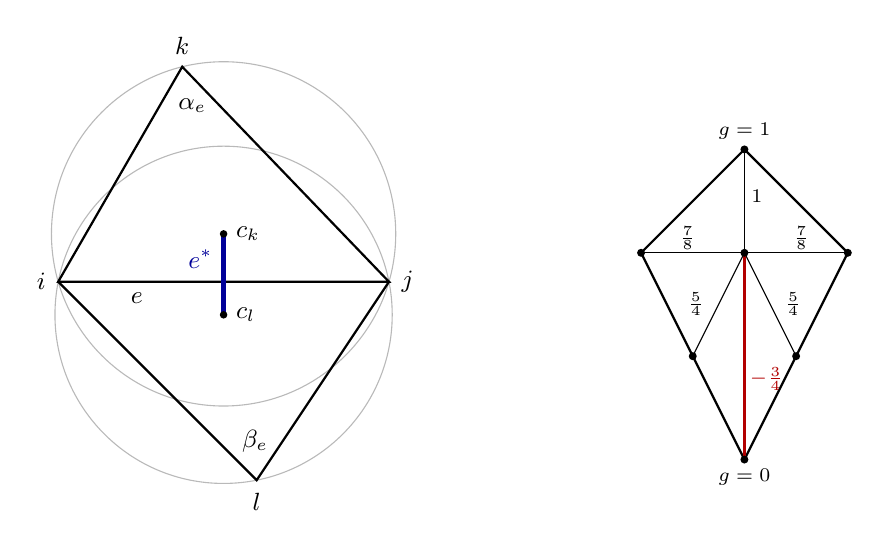
\begin{tikzpicture}[scale=1.05,>=stealth]
  % left: an interior edge with its dual segment
  \coordinate (i) at (0,0); \coordinate (j) at (4,0);
  \coordinate (k) at (1.5,2.6); \coordinate (l) at (2.4,-2.4);
  \coordinate (ck) at (2,0.5788); \coordinate (cl) at (2,-0.4);
  \draw[gray!55] (ck) circle (2.0821);
  \draw[gray!55] (cl) circle (2.0396);
  \draw[thick] (i)--(j)--(k)--cycle; \draw[thick] (i)--(l)--(j);
  \draw[line width=1.6pt,blue!60!black] (cl)--(ck);
  \fill (ck) circle (1.3pt) node[right=1pt,font=\small] {$c_k$};
  \fill (cl) circle (1.3pt) node[right=1pt,font=\small] {$c_l$};
  \node[left=1pt,font=\small] at (i) {$i$}; \node[right=1pt,font=\small] at (j) {$j$};
  \node[above=1pt,font=\small] at (k) {$k$}; \node[below=1pt,font=\small] at (l) {$l$};
  \node[font=\small] at (1.62,2.13) {$\alpha_e$}; \node[font=\small] at (2.38,-1.93) {$\beta_e$};
  \node[font=\small] at (0.95,-0.2) {$e$}; \node[font=\small,blue!60!black] at (1.72,0.27) {$e^*$};
  % right: the hexagon of Example 2.4
  \begin{scope}[shift={(8.3,0.35)},scale=1.25]
    \coordinate (o) at (0,0);
    \coordinate (a) at (-0.5,-1); \coordinate (b) at (0,-2); \coordinate (c) at (0.5,-1);
    \coordinate (d) at (1,0); \coordinate (f) at (0,1); \coordinate (g) at (-1,0);
    \draw[thick] (a)--(b)--(c)--(d)--(f)--(g)--cycle;
    \foreach \p in {a,c,d,f,g} \draw (o)--(\p);
    \draw[red!70!black,very thick] (o)--(b);
    \foreach \p in {o,a,b,c,d,f,g} \fill (\p) circle (1.1pt);
    \node[font=\scriptsize,red!70!black] at (0.215,-1.22) {$-\frac34$};
    \node[font=\scriptsize] at (-0.47,-0.5) {$\frac54$}; \node[font=\scriptsize] at (0.47,-0.5) {$\frac54$};
    \node[font=\scriptsize] at (0.55,0.14) {$\frac78$}; \node[font=\scriptsize] at (-0.55,0.14) {$\frac78$};
    \node[font=\scriptsize] at (0.12,0.55) {$1$};
    \node[font=\scriptsize,below] at (b) {$g=0$};
    \node[font=\scriptsize,above] at (f) {$g=1$};
  \end{scope}
\end{tikzpicture}
\caption{Left: an interior edge $e$, the opposite angles, and the dual segment $e^*$ joining the two circumcenters; $w_e=|e^*|/|e|$.
Right: the triangulation of Example~\ref{ex:hex} with the conductances at the interior vertex; the red edge is not locally Delaunay.}
\label{fig:one}
\end{figure}

\begin{proposition}[The weight is a ratio of dual to primal length]\label{prop:dual}
Let $e=ij$ be an interior edge shared by the triangles $ijk$ and $ijl$, with circumcenters $c_k$ and $c_l$, and let $\nu$ be the unit normal
to $e$ pointing to the side of $k$. Then
\[
w_e=\frac{\langle c_k-c_l,\nu\rangle}{|e|}=:\frac{|e^*|_{\pm}}{|e|},
\]
the signed length of the dual segment $e^*=c_lc_k$ divided by the length of $e$. For a boundary edge the same holds with $c_l$ replaced by the
midpoint of $e$.
\end{proposition}

\begin{proof}
Both circumcenters lie on the perpendicular bisector of $e$. The edge $e$ subtends the angle $2\alpha_e$ at $c_k$, so the signed
distance from the midpoint $m$ of $e$ to $c_k$, measured towards $k$, is $\frac{|e|}2\cot\alpha_e$; it is negative precisely when
$\alpha_e>\pi/2$. Likewise $\langle c_l-m,-\nu\rangle=\frac{|e|}{2}\cot\beta_e$. Add.
\end{proof}

So $w_e$ is the conductance of a rectangular strip of unit-conductivity material of length $|e|$ and width $|e^*|$: on a
Delaunay triangulation the piecewise-linear finite element method coincides with the finite-volume method on the dual Voronoi
cells.

\begin{corollary}[Sign of the weights]\label{cor:sign}
For an interior edge put $\theta_e:=\pi-\alpha_e-\beta_e$. Then
\[
w_e=\frac{\sin(\alpha_e+\beta_e)}{2\sin\alpha_e\sin\beta_e}=\frac{\sin\theta_e}{2\sin\alpha_e\sin\beta_e},
\]
and $w_e>0$, $=0$, $<0$ according as $l$ lies outside, on, or inside the circumcircle of $ijk$: $w_e\ge0$ if and only if $e$ is
\emph{locally Delaunay}. For a boundary edge, $w_e\geq0$ if and only if $\alpha_e\le\pi/2$, that is, if and only if the opposite vertex does not lie inside
the circle having $e$ as a diameter.
\end{corollary}

\begin{remark}\label{rem:theta}
The number $\theta_e$ is the exterior intersection angle of the two circumcircles, equivalently the exterior dihedral angle at $e$ of the ideal
hyperbolic polyhedron attached to the triangulation \cite{Riv94}. Prescribing the $\theta_e$ and asking for the triangulation is Rivin's problem, taken up in Section~\ref{sec:volume}, where $w_e$ reappears as an entry of a Hessian.
A different question is whether a \emph{combinatorial} triangulation admits Delaunay angles at all, with the $\theta_e\ge0$ as unknowns. That is a linear-programming
feasibility question in which each angle variable enters three constraints (its triangle, its vertex, its opposite edge); the linear systems that
interior-point methods generate for it are not diagonally dominant, so the solvers of Section~\ref{sec:solve} do not apply to it directly. With prescribed $\theta_e$ the corresponding problem is a planar flow problem (Remark~\ref{rem:lp}).
\end{remark}

\section{The discrete Dirichlet problem}\label{sec:dirichlet}

Given $g\colon B\to\R$, minimize $D(u)$ over $u\in\PL(\cT)$ with $u|_B=g$. Write $L$ in block form with respect to $V=I\sqcup B$.

\begin{proposition}[Valid for every triangulation]\label{prop:any}
\textup{(a)} $L$ is positive semidefinite with kernel the constants, and $L_{II}$ is positive definite. The minimizer is unique and is given by
\begin{equation}\label{eq:system}
L_{II}\,u_I=-L_{IB}\,g,\qquad\text{that is,}\qquad \sum_jw_{ij}(u_i-u_j)=0\quad\text{for every } i\in I ,
\end{equation}
which is Kirchhoff's current law at the interior nodes.
\textup{(b)} \emph{Linear precision:} if $g$ is the restriction of an affine function, then $u$ is that affine function. In particular
$\sum_jw_{ij}(p_i-p_j)=0$ for $i\in I$.
\end{proposition}

\begin{proof}
(a) $u^{\mathsf T}Lu=\int_\Omega|\nabla u|^2\ge0$, with equality only for constants because $\Omega$ is connected.
(b) An affine function is harmonic, so it minimizes the Dirichlet integral among all $H^1$ functions with its boundary values, and in particular
among the piecewise-linear ones.
\end{proof}

\begin{proposition}[Nonnegative conductances]\label{prop:pos}
Suppose that $w_e\ge0$ for every edge having at least one endpoint in $I$. Then every interior vertex is joined to $B$ by a path of edges of positive
weight (otherwise the indicator function of a set of interior vertices would have zero energy, contradicting Proposition~\ref{prop:any}(a)), and:
\begin{enumerate}[label=\textup{(\alph*)},leftmargin=*]
\item $L_{II}$ is a nonsingular Stieltjes matrix: symmetric, with nonpositive off-diagonal entries, weakly diagonally dominant, and $L_{II}^{-1}\ge0$ entrywise.
In the terminology of \cite{STsolve} it is an SDDM matrix.
\item Each $u_i$, $i\in I$, is a weighted average of the neighbouring values with nonnegative weights. Hence the discrete maximum principle holds:
$\min g\le u\le\max g$.
\item $u_i=\E_i\,g(X_\tau)$, where $X$ is the random walk with transition probabilities $w_{ij}/\sum_kw_{ik}$ and $\tau$ is the hitting time of $B$. The
$i$-th row of $-L_{II}^{-1}L_{IB}$ is the harmonic measure on $B$ seen from $i$. By Proposition~\ref{prop:any}(b) the walk is a martingale: every interior
vertex is the $w$-weighted barycenter of its neighbours.
\item The whole dictionary between reversible random walks and electrical networks applies \cite{DS84}: effective resistance, Dirichlet's and Thomson's principles, and
Rayleigh monotonicity.
\end{enumerate}
\end{proposition}

\begin{remark}[Which edges matter]\label{rem:which}
An edge joining two boundary vertices contributes a constant to $D(u)$ and enters neither $L_{II}$ nor $L_{IB}$. For the Dirichlet
problem, therefore, the hypothesis of Proposition~\ref{prop:pos} concerns interior edges only, and it says that those with an interior endpoint are
locally Delaunay. If all interior edges are locally Delaunay, then $\cT$ is a Delaunay triangulation of its vertex set, constrained by $\partial\Omega$ when
$\Omega$ is not convex (Delaunay's lemma). For Neumann, mixed, or eigenvalue problems all of $L$ matters, and nonnegativity of the boundary weights
requires in addition that $\alpha_e\le\pi/2$ on boundary edges, which is the ``boundary-conforming Delaunay'' condition of the meshing literature.
\end{remark}

\begin{example}[Failure of the maximum principle]\label{ex:hex}
Let $\Omega$ be the kite with vertices $(0,-2)$, $(1,0)$, $(0,1)$, $(-1,0)$, place two further boundary vertices at the midpoints $(\pm\frac12,-1)$ of its lower sides, and cone
the resulting hexagon from the origin (Figure~\ref{fig:one}, right). The
edge from the origin to $(0,-2)$ has opposite angles $\alpha=\beta=\pi-2\arctan\frac12>\frac\pi2$ and weight $\cot\alpha=-\frac34$; the other five weights are
$\frac54,\frac54,\frac78,\frac78,1$, with total $\frac92$. With $g=0$ at $(0,-2)$ and $g=1$ at the other five boundary vertices, \eqref{eq:system} gives
\[
u(0)=\bigl(\tfrac52+\tfrac74+1\bigr)\big/\tfrac92=\tfrac76>1 .
\]
Flipping the offending edge produces the Delaunay triangulation, with weights $\frac12,\frac12,\frac78,\frac78,1$ at the origin and $u(0)=1$.
\end{example}

\begin{remark}[What is lost without Delaunay, and what is not]\label{rem:lost}
For an arbitrary triangulation the system \eqref{eq:system} is still symmetric positive definite, $u$ is still the energy minimizer, and
the energy-norm error analysis of Section~\ref{sec:conv} is unaffected. What is lost is the maximum principle, the probabilistic and network
interpretation, and the diagonal dominance of $L_{II}$ on which the solvers of Section~\ref{sec:solve} rely.
\end{remark}

\section{Delaunay triangulations are optimal}\label{sec:rippa}

\begin{theorem}[Rippa \cite{Rip90}]\label{thm:rippa}
Let $\cT$ be any triangulation of the convex hull of a finite set $V\subset\R^2$ with vertex set $V$, and let $\cT_D$ be a Delaunay triangulation of $V$.
Then $D_{\cT_D}(u)\le D_{\cT}(u)$ for every $u\in\R^V$; in other words
\[
L(\cT_D)\lo L(\cT)
\]
in the Loewner order. More precisely, if two triangulations differ by the flip of one edge inside a convex quadrilateral $Q$, and $\lambda$ denotes the linear
functional on $\R^{\mathrm{vert}(Q)}$ \textup{(}unique up to scale\textup{)} that vanishes on restrictions of affine functions, then the two matrices differ by
$c\,\lambda\lambda^{\mathsf T}$ with $c\ge0$, the smaller matrix belonging to the locally Delaunay diagonal. One has $c=0$ exactly when the four points are concyclic.
\end{theorem}

The flip statement is a direct computation. The global statement follows because Lawson's algorithm, which flips edges that are not locally Delaunay for as long as there are any,
reaches $\cT_D$ from any $\cT$: an edge with $\alpha_e+\beta_e>\pi$ lies in a strictly convex quadrilateral, so it can be flipped,
and each flip strictly decreases $D(u)$ for $u=|x|^2$, so the process terminates.

\begin{corollary}
For fixed vertex set and boundary data, $\min\{D_{\cT}(u):u|_B=g\}$ is smallest for the Delaunay triangulation.
By Dirichlet's principle each of these minima bounds from above the energy of the harmonic function with the piecewise-linear boundary values $g$,
so the Delaunay network gives the best such upper bound available from the given vertices.
For a non-convex polygon the same holds with the constrained Delaunay triangulation, since flips never touch the boundary edges.
\end{corollary}

Two comments. First, ``Delaunay'' is not a restriction on the vertex set. It is a choice of triangulation of a given vertex set, which can be computed in $O(n\log n)$ time,
also in the constrained version needed for non-convex polygons \cite{Chew89}. Second, the statement is intrinsic. Delaunay triangulations exist on every piecewise flat surface \cite{Riv94,ILTC01}. Bobenko and Springborn \cite{BS07} prove that the Delaunay tessellation is unique,
observe that Rippa's argument carries over to piecewise flat surfaces and use it to show that the flip algorithm terminates there as well, and define the
discrete Laplace--Beltrami operator of the surface by the cotangent weights of its intrinsic Delaunay triangulation, which are nonnegative.

\section{Convergence}\label{sec:conv}

\subsection{Energy norm}
Let $\Omega$ be a convex polygon, $g$ the restriction to $\partial\Omega$ of a function in $H^2(\Omega)$, $u$ the harmonic extension (so $u\in H^2(\Omega)$ by convexity),
and $u_h\in\PL(\cT)$ the solution of \eqref{eq:system} with the nodal values of $g$. Both $u$ and $u_h$ are $D$-orthogonal to the piecewise-linear functions vanishing on
$\partial\Omega$, and $I_hu-u_h$ is such a function, $I_h$ being nodal interpolation. Hence
\begin{equation}\label{eq:cea}
|u-u_h|_{H^1(\Omega)}\le|u-I_hu|_{H^1(\Omega)}\le C(\gamma)\,h\,|u|_{H^2(\Omega)},
\end{equation}
where $h$ is the largest edge length and $\gamma<\pi$ is an upper bound for all angles of all triangles. The first inequality is C\'ea's lemma.
The second is the interpolation estimate under the \emph{maximum angle condition} of Synge and Babu\v{s}ka--Aziz \cite{BA76}; small angles do no harm, but angles near $\pi$ do.
The Delaunay property plays no role here. If $\Omega$ has a re-entrant corner of interior angle $\omega>\pi$, then $u$ contains a multiple of $r^{\pi/\omega}\sin(\pi\phi/\omega)$ and does not belong to $H^2$;
on quasi-uniform meshes the rate drops to about $h^{\pi/\omega}$, and graded meshes are needed to restore it.

\subsection{Uniform convergence}
When the weights are nonnegative, the maximum principle gives stability in the sup norm. Ciarlet and Raviart \cite{CR73} used it to prove uniform convergence for regular families of
non-obtuse triangulations. For Delaunay triangulations without angle bounds, the natural framework goes back to another paper of Duffin \cite{Duf68}, on discrete analytic functions on rhombic lattices. As Duffin already observed, what the theory needs is a planar
quadrilateral graph whose faces have orthogonal diagonals, the conductance of a diagonal being the length of the other diagonal divided by its own; with these weights the coordinate functions are discrete harmonic (compare Proposition~\ref{prop:any}(b)).
By Proposition~\ref{prop:dual}, a Delaunay triangulation together with its circumcenters is such a graph. Its quadrilaterals are the kites $i\,c_l\,j\,c_k$,
which need not be convex, and its conductances are the cotangent weights.

\begin{itemize}[leftmargin=*]
\item Skopenkov \cite{Sko13} proved uniform convergence of the discrete Dirichlet solution on such ``orthogonal lattices'' for smooth boundary data on bounded simply connected domains, under two
regularity hypotheses: in each face the ratio of the diagonals is bounded, and the number of vertices in any disk of radius equal to the maximal edge length is bounded.
He deduces uniform convergence of the finite element method on Delaunay triangulations, which had been posed as a problem by Bobenko. Werness \cite{Wer15} removed the second, global, hypothesis, at the cost of a slightly different local one.
\item Gurel-Gurevich, Jerison and Nachmias \cite{GJN20} removed all regularity hypotheses and made the bound effective. Let $\Omega$ be a bounded simply connected domain and $g\in C^2(\R^2)$. If $G$ is an ``orthodiagonal map'' with maximal edge length at most $\eps$, and
$\partial G$ is within Hausdorff distance $\delta$ of $\partial\Omega$, then at every primal vertex in $\overline\Omega$
\[
|u_{\mathrm{discrete}}-u|\;\le\;\frac{C\,\diam(\Omega)\,\bigl(\|\nabla g\|_\infty+\eps\,\|\nabla^2g\|_\infty\bigr)}{\log^{1/2}\bigl(\diam(\Omega)/(\delta\vee\eps)\bigr)}
\]
with a universal constant $C$, the norms being suprema over the convex hull of $\overline\Omega$ and the map.
\end{itemize}

In the Delaunay dictionary the edges of the orthodiagonal map are the segments joining each vertex to the circumcenters of its incident triangles. The mesh parameter $\eps$ in these theorems
is therefore the largest \emph{circumradius}, not the largest edge length. Near $\partial\Omega$ this matters: a boundary triangle with a large angle opposite its boundary edge has a distant circumcenter, and the boundary-conforming
condition of Remark~\ref{rem:which} is what keeps $\eps$ and $\delta$ small there. (At the boundary the quadrilateral structure is completed by one auxiliary dual vertex per boundary edge, placed on its perpendicular bisector just outside $\Omega$; this is the device of \cite[Proposition~2.1]{GJN20}. The corresponding
weights are irrelevant by Remark~\ref{rem:which}; for the precise hypotheses in the finite element setting see \cite[Cor.~5.1]{Sko13}.) The logarithmic rate is the price of assuming nothing about the mesh. For smooth solutions on quasi-uniform meshes the classical sup-norm rate is $O(h^2|\log h|)$.

\section{Hyperbolic volume: the same matrix as a Hessian}\label{sec:volume}

The angles $\theta_e$ of Remark~\ref{rem:theta} are the data of a second variational problem on the same triangulation, and the cotangent matrix reappears there as a Hessian.
In this section and the next, $\Delta_e:=\alpha_e+\beta_e=\pi-\theta_e$ denotes the \emph{interior dihedral angle} at an interior edge, and $\Delta_e:=\alpha_e$ at a boundary edge.
By Corollary~\ref{cor:sign}, $w_e=\sin\Delta_e/(2\sin\alpha_e\sin\beta_e)$.

\subsection{Rivin's variational principle}
Regard the plane as the boundary of the upper half-space model of $\mathbb H^3$. If $\cT$ is a Delaunay triangulation, the ideal polyhedron $P_\cT$ spanned by $V\cup\{\infty\}$ is convex and is the union of the ideal tetrahedra $\infty ijk$
over the triangles $ijk$ of $\cT$. The dihedral angles of $\infty ijk$ at its three vertical edges are the angles of the triangle $ijk$, opposite edges of an ideal tetrahedron have equal dihedral angles, and the volume of $\infty ijk$ is
$\Lambda(\alpha)+\Lambda(\beta)+\Lambda(\gamma)$, where $\Lambda(x)=-\int_0^x\log|2\sin t|\,dt$ is the Lobachevsky function \cite{Mil82}. Consequently the dihedral angle of $P_\cT$ at a finite edge $e$ is $\Delta_e$, and
\[
\operatorname{vol}(P_\cT)=\mathcal V(\alpha):=\sum_{c}\Lambda(\alpha_c),
\]
the sum being over the corners $c$ of the triangles.

Rivin's problem \cite{Riv94,Riv96} is the inverse one: given a combinatorial triangulation $\cT$ and a function $\Delta\colon E\to(0,\pi]$, find a Delaunay triangulation with dihedral angles $\Delta$
(an edge with $\Delta_e=\pi$ is not an edge of the polyhedron, whose faces therefore need not be triangles).
An \emph{angle structure} is an assignment of angles $\alpha_c\in(0,\pi)$ to the corners such that the angles of every triangle add up to $\pi$ and the angles opposite every edge add up to $\Delta_e$.
Angle structures form the relative interior $\mathcal P(\Delta)$ of a convex polytope given by $|F|+|E|$ linear equations and $3|F|$ inequalities. In every angle structure the angles at an interior vertex $i$ add up to $\sum_{e\ni i}\theta_e$,
so $\sum_{e\ni i}\theta_e=2\pi$ is a necessary condition on the data, assumed from now on.

\begin{theorem}[Rivin \cite{Riv94}]\label{thm:rivin}
The function $\mathcal V$ is strictly concave on $\mathcal P(\Delta)$. If $\mathcal P(\Delta)\neq\emptyset$, then $\mathcal V$ attains its maximum over the closed polytope at a unique point $\alpha^*$, which lies in $\mathcal P(\Delta)$ and is the system of angles of a
Delaunay triangulation with dihedral angles $\Delta$; this triangulation is unique up to similarity.
\end{theorem}

\begin{theorem}[Rivin \cite{Riv96}]\label{thm:ideal}
A polyhedral graph with weights $\theta_e\in(0,\pi)$ on its edges is the $1$-skeleton of a convex ideal polyhedron with exterior dihedral angles $\theta_e$
if and only if $\sum_{e\ni v}\theta_e=2\pi$ at every vertex $v$ and $\sum_{e\in C}\theta_e>2\pi$ for every simple circuit $C$ of the dual graph that does not bound a dual face. The polyhedron is unique up to isometry.
\end{theorem}

The two theorems have different origins. Theorem~\ref{thm:ideal} was not proved by a variational method. It was derived in \cite{Riv96} from the characterization of \emph{compact} convex hyperbolic polyhedra by their dual metrics, which is Rivin's theorem (his thesis \cite{RivTh}, published in \cite{HR93}):
a metric on the sphere is the dual metric of a compact convex polyhedron if and only if it is spherical with cone points of angle greater than $2\pi$ and all its closed geodesics are longer than $2\pi$. The ideal case follows by a limiting argument,
together with a proof that for ideal polyhedra the closed geodesics of the dual metric correspond to circuits of the dual graph; this is how the circuit inequalities arise.
The variational approach of \cite{Riv94} leads instead to the question whether $\mathcal P(\Delta)$ is empty. That is a linear program of polynomial size, much smaller than the exponentially large family of circuit inequalities, and in \cite{Riv03} it is reduced to a network flow problem (Remark~\ref{rem:lp}).
That the circuit inequalities are the conditions dual to this linear program was observed by Andrew Casson. The two strands joined in what is now called the Casson--Rivin program for ideal triangulations of $3$-manifolds \cite{FG11}, and \cite{Riv03} also shows that there the analogues of the obstructing circuits are normal surfaces of genus $0$ and $1$ (Section~\ref{sec:context}).

To pass from Theorem~\ref{thm:ideal} to the setting of Theorem~\ref{thm:rivin}, send one vertex of the polyhedron to $\infty$ and triangulate the faces: $\cT$ is what remains after the star of $\infty$ is deleted, the boundary edges of $\cT$ carry the dihedral angles $\Delta_e=\pi-\theta_e$
that the finite faces make with the vertical ones, and the circuit inequalities are equivalent to $\mathcal P(\Delta)\ne\emptyset$.

\subsection{Coordinates, gradient, Hessian}
Orient every triangle positively, so that each of its edges acquires a direction, and say that the corner $c$ of the triangle $ijk$ at $k$ is \emph{opposite the directed edge} $i\to j$.

\begin{proposition}\label{prop:hessian}
Fix an angle structure $\alpha^0$ and, for $u\in\R^V$, put $\alpha_c(u)=\alpha^0_c+u_i-u_j$ when $c$ is opposite the directed edge $i\to j$.
\begin{enumerate}[label=\textup{(\alph*)},leftmargin=*]
\item $\alpha(u)$ satisfies all the linear equations of an angle structure with the same $\Delta$ at interior edges, and leaves the angles opposite boundary edges unchanged if and only if $u$ is constant on $B$.
If $\cT$ is a disk, the map $u\mapsto\alpha(u)$, $u|_B=0$, is an affine isomorphism of $\R^I$ onto the affine hull of $\mathcal P(\Delta)$.
\item $\partial\mathcal V/\partial u_i=\log H_i$, where $H_i=\prod_{t\ni i}\sin\alpha_{t,j}/\sin\alpha_{t,k}$, the product being over the positively oriented triangles $t=ijk$ around $i$ and $\alpha_{t,j}$ denoting the angle of $t$ at $j$. By the law of sines $H_i$ is the dilation accumulated on developing the triangles with angles $\alpha(u)$ once
around $i$. Thus $\nabla\mathcal V=0$ says precisely that the triangles fit together.
\item $\operatorname{Hess}_u\mathcal V=-2\,L_{II}(\alpha(u))$, where $L(\alpha)$ is the cotangent matrix of Section~\ref{sec:cotan} formed with the current angles. Its weights satisfy
\begin{equation}\label{eq:wlower}
w_e(\alpha)=\frac{\sin\Delta_e}{2\sin\alpha_e\sin\beta_e}\;\ge\;\cot\frac{\Delta_e}2\;\ge0
\end{equation}
for \emph{every} angle structure, geometric or not.
\end{enumerate}
\end{proposition}

\begin{proof}
(a) In the triangle $ijk$ the three increments are $u_i-u_j$, $u_j-u_k$, $u_k-u_i$, with sum zero. An interior edge $ij$ is directed $i\to j$ in one of its triangles and $j\to i$ in the other, so the two increments opposite to it cancel. At a boundary edge $ij$ the increment is $\pm(u_i-u_j)$.
The map is injective because the $1$-skeleton is connected, and the dimensions agree: for a disk, Euler's formula gives $3|F|-|F|-|E|=|I|-1$, and the equations have exactly one linear relation (the sum of the triangle equations equals the sum of the edge equations).
(b) and (c) follow from $\Lambda'(x)=-\log(2\sin x)$ and $\Lambda''(x)=-\cot x$ by the chain rule: the two corners opposite an edge $e=ij$ contribute $-(\cot\alpha_e+\cot\beta_e)(u_i-u_j)^2=-2w_e(u_i-u_j)^2$ to the second differential.
Finally $2\sin\alpha_e\sin\beta_e=\cos(\alpha_e-\beta_e)-\cos\Delta_e\le2\sin^2(\Delta_e/2)$.
\end{proof}

The coordinate vector of $u=\mathbf 1_i$ adds $\eps$ to one base angle and subtracts it from the other in every triangle around $i$. By (a) these deformations span the tangent space of $\mathcal P(\Delta)$ (compare \cite{Riv94}); they are the two-dimensional counterpart of the
leading--trailing deformations of angled ideal triangulations of $3$-manifolds \cite{FG11}.
Several consequences are worth stating.

\emph{The stiffness matrix is a Hessian of volume.} At $\alpha^*$ the matrix $L(\alpha^*)$ is the piecewise-linear finite element stiffness matrix of the realized Delaunay triangulation, so $K=-\frac12\operatorname{Hess}\mathcal V$ there.
To first order, $\log H=-2L_{II}u$: the discrete Laplacian of $u$ measures the failure of the deformed triangles to close up.

\emph{Positivity is automatic.} In Section~\ref{sec:dirichlet} nonnegativity of the conductances was a property of a particular mesh. Here it holds at every point of $\mathcal P(\Delta)$, because the dihedral angles are data and never change. No flips occur: the combinatorics are fixed,
and intermediate angle structures are not geometric.

\emph{Uniform strong concavity.} If $\Delta_e\le\theta_{\max}<\pi$ for all $e$, then by \eqref{eq:wlower}
\[
-d^2\mathcal V\;\ge\;\cot(\theta_{\max}/2)\,|d\alpha|^2\qquad\text{on all of }\mathcal P(\Delta).
\]
Hence an angle structure whose volume is within $\eta$ of the maximum is within
$\sqrt{2\eta\tan(\theta_{\max}/2)}$ of $\alpha^*$ in the Euclidean norm of $\R^{3|F|}$. Only the \emph{upper} bound on the Hessian degenerates, at the boundary of the polytope, where some $\cot\alpha_c\to\infty$.

\emph{Newton's method is a sequence of Duffin problems.} The Newton iteration for maximizing $\mathcal V$ is
\begin{equation}\label{eq:newton}
2\,L_{II}(\alpha(u))\,\delta=\log H(u),\qquad u\leftarrow u+\delta .
\end{equation}
Each step is a discrete Poisson problem on the resistor network of Sections~\ref{sec:cotan}--\ref{sec:dirichlet}, with the conductances of the current angle structure, zero boundary values, and current $\frac12\log H_i$ injected at the vertex $i$.
The matrix is of the kind required in Section~\ref{sec:solve}. In a numerical test (a Delaunay triangulation of $40$ random points, the angle structure perturbed by a random $u$ of size one fifth of the smallest angle)
the iteration \eqref{eq:newton} returned to $\alpha^*$ with $|\nabla\mathcal V|_\infty=4\cdot10^{-1},\,3\cdot10^{-2},\,2\cdot10^{-4},\,3\cdot10^{-9},\,2\cdot10^{-15}$.

\begin{remark}[The dual principle is the dual network]\label{rem:BS}
Bobenko and Springborn \cite{BS04} solve the same problem by minimizing a convex function $S(\rho)$ of the logarithms $\rho_f$ of the circumradii, one variable per triangle, defined on all of $\R^F$ with no inequality constraints; they show that Rivin's functional is obtained from theirs by a Legendre transformation.
Its second differential is $\sum_e\frac{\sin\theta_e}{\cosh(\rho_f-\rho_{f'})-\cos\theta_e}(d\rho_f-d\rho_{f'})^2$, the sum being over interior edges $e=f\cap f'$. For a geometric configuration one checks that
\[
\frac{\sin\theta_e}{\cosh(\rho_f-\rho_{f'})-\cos\theta_e}=\frac{2\sin\alpha_e\sin\beta_e}{\sin\theta_e}=\frac1{w_e}=\frac{|e|}{|e^*|}
\]
(use $r_f\sin\alpha_e=r_{f'}\sin\beta_e=|e|/2$). So the Hessian of the dual functional is the Laplacian of the \emph{dual} network, on the Voronoi graph, with the reciprocal conductances: the two variational principles correspond to the two networks of Duffin's
orthodiagonal structure (Section~\ref{sec:conv}). These weights are positive for all $\rho$, and their logarithmic derivative in $\rho_f-\rho_{f'}$ is bounded by $\max(1,1/\sin\theta_e)$.
\end{remark}

\begin{remark}[Two families out of three: planar flow]\label{rem:lp}
A point of $\mathcal P(\Delta)$ has to be found first. Each angle variable occurs in exactly two equations, that of its triangle and that of its opposite edge, so the constraint matrix $A$ is the unsigned incidence matrix of a bipartite planar graph $\Gamma$
(triangles on one side, edges on the other, corners as arcs). This is a transportation problem: every triangle ships $\pi$, the edge $e$ receives $\Delta_e$, and the angle $\alpha_c$ is the flow in the arc $c$. Finding a point of $\mathcal P(\Delta)$, with a prescribed margin $\alpha_c\ge s$ if desired,
is therefore a flow-feasibility problem on a planar graph. This reduction is carried out in \cite{Riv03}, and the cut conditions of the flow problem are the circuit inequalities of Theorem~\ref{thm:ideal}, as observed by Casson. It can be solved in nearly linear time outright, by the planar maximum-flow algorithm for several sources and sinks \cite{BKMNW17} or by the $\Ot(n)$ algorithm for planar minimum-cost flow
\cite{DGGLPSY22}; one does not even need an interior-point method whose normal equations $ADA^{\mathsf T}=D_\Gamma+W_\Gamma$ happen to be Laplacian after a change of sign on one side of the bipartition, although that is also true.

The general principle is that a corner angle occurs in three linear forms: the sum over its triangle \textup{(T)}, the sum at its vertex \textup{(V)}, and the sum opposite its edge \textup{(E)}. Any two of the three families give a bipartite incidence matrix, hence a planar flow problem;
this applies to \textup{(T,\,E)}, which is Rivin's problem, and equally to \textup{(T,\,V)}. All three together, as in the linear program of Remark~\ref{rem:theta} where the dihedral angles are unknowns subject to $\alpha_e+\beta_e\le\pi$, give the incidence matrix $A_3$ of a $3$-uniform tripartite hypergraph, and
$A_3DA_3^{\mathsf T}=\sum_cd_c\,(e_{t}+e_{v}+e_{e})(e_{t}+e_{v}+e_{e})^{\mathsf T}$ has nonnegative off-diagonal entries along the odd cycles $t,v,e$. No change of signs or diagonal scaling makes it diagonally dominant (it has factor width three, and factor width two characterizes the matrices that can be so scaled \cite{BCPT05}).
The step from two entries per column to three is the step from flows to general linear programs: two-commodity flow is already equivalent to linear programming \cite{DKZ22}. Our instances are special, so this is context and not a lower bound.

Moving one family from the constraints into the objective does not help by itself. Minimizing $\sum_v(\sum_{c\ni v}\alpha_c-2\pi)^2$ subject to \textup{(T)} and \textup{(E)} is a convex quadratic program, and minimizing $\max_e(\alpha_e+\beta_e)$ subject to \textup{(T)} and \textup{(V)} is a linear program, but a penalty is a regularized constraint: with the residuals as auxiliary
variables the normal matrix of the first is $A_3DA_3^{\mathsf T}$ plus a positive diagonal on the vertex block, which leaves the rows of the triangles as far from diagonal dominance as before. In the second the edge constraints remain, and the new variable occurs in all of them, a dense column, so that one should bisect on its value instead.
What these formulations do provide is robustness: they always have interior points, the optimal value is a certificate (a maximum below $\pi$, or a sum of squares equal to zero), and for unrealizable data they measure the distance to realizability.
For the three-family problem the bounds that are available do not use Laplacian structure. The hypergraph of $A_3$ can be drawn inside the triangulation with a bounded number of crossings per edge, so it has separators of size $O(\sqrt n)$ in the sense required by \cite{DGLSY24}, whose Theorem~1.2 then gives the running time
$\Ot(n^{3/2}\log(R/(r\eps)))$, where $r$ is the inner radius of the polytope and $R$ the size of the box bounding the variables; interior-point iterations with nested dissection give $\Ot(n^{(1+\omega)/2})$, about $n^{1.69}$. Note that $n^{3/2}$ is also what $\sqrt n$ iterations with nearly-linear-time solves would give.
The reason flows do better is that there the matrices $ADA^{\mathsf T}$ and all their Schur complements along a separator tree are Laplacians, which can be sparsified \cite{DGGLPSY22}; that is exactly what a third entry per column destroys.
One can also alternate between the two flow problems \textup{(T,\,E)} and \textup{(T,\,V)}, each step costing $\Ot(n)$, but no polylogarithmic bound on the number of steps is available for such splitting methods.
\end{remark}

\begin{remark}[Vertex sums as the equation: Thurston's algorithm, Ricci and Calabi flows]\label{rem:thurston}
A Delaunay realization has to satisfy \textup{(T)}, \textup{(E)}, \textup{(V)} and the gluing condition \textup{(G)} that the triangles fit together. The variational principles differ in which of these conditions are built into the variables and which one is left as the equation.
In Rivin's principle the variables are angles, \textup{(T)} and \textup{(E)} hold on $\mathcal P(\Delta)$ and imply \textup{(V)}, and \textup{(G)} is the equation $\nabla\mathcal V=0$. In the principle of Bobenko and Springborn (Remark~\ref{rem:BS}) the variables are the radii of the circles of the faces,
\textup{(E)} and \textup{(G)} are built in, and the equation is that the angles around the centre of each circle add up to $2\pi$, which is \textup{(T)}.
In Thurston's algorithm for circle packings \cite{CS03} the variables are the radii $r_v$ of circles centred at the \emph{vertices} of a triangulation. The triangle on three vertices has sides $r_i+r_j$ (or the sides determined by prescribed intersection angles), so \textup{(T)}, \textup{(E)} and \textup{(G)} hold identically, in a piecewise flat metric with cone points,
and the equations are the vertex sums: the curvatures $K_v=2\pi-\sum_{c\ni v}\alpha_c$ must vanish. Thurston's iteration adjusts one radius at a time so as to make $K_v=0$, using the monotonicity of the angle sum in $r_v$.
With $u_v=\log r_v$ the map $u\mapsto K$ is the gradient of a convex function, the functional of Colin de Verdi\`ere \cite{CdV91}, which can also be derived from that of \cite{BS04}; its gradient flow $\dot u_v=-K_v$ is the combinatorial Ricci flow of Chow and Luo \cite{CL03}, and Thurston's algorithm is coordinate-wise relaxation for the same convex function.
The sum of squares $\sum_vK_v^2$ considered in Remark~\ref{rem:lp} is, in these variables, the combinatorial Calabi energy, and its gradient flow $\dot u=-(\partial K/\partial u)K$ is the combinatorial Calabi flow \cite{Ge18}.
So relaxing the vertex equations and driving the curvatures to zero is Thurston's idea. In the variables $r_v$ the intersection angles are data and the problem is nonlinear with a convex potential; in the angle variables the dihedral angles may be left free, subject to $\alpha_e+\beta_e\le\pi$, and the problem is a convex quadratic program, whose solution is an angle structure and still has to be made geometric by Section~\ref{sec:volume}.

The linear algebra is the same once more. For tangent circles one computes
\[
\frac{\partial K_i}{\partial u_j}=-\frac{\varrho_t+\varrho_{t'}}{r_i+r_j}\quad(j\sim i),\qquad \frac{\partial K_i}{\partial u_i}=\sum_{j\sim i}\frac{\varrho_t+\varrho_{t'}}{r_i+r_j},
\]
where $\varrho_t,\varrho_{t'}$ are the inradii of the two triangles on the edge $ij$. The incircle of a triangle of centres passes through the three points of tangency, so $\varrho_t+\varrho_{t'}=|e^*|$ is the distance between the two incentres, and the conductance is again $|e^*|/|e|$, for the orthogonal dual structure formed by the incentres.
These conductances are positive for all radii. Newton's method for the packing equations is therefore also a sequence of Dirichlet problems on planar resistor networks, to which Section~\ref{sec:solve} applies, and the linearized packing algorithm of \cite{OSC17} likewise alternates sparse linear solves with updates of the radii.
\end{remark}

\begin{remark}[$\mathcal V$ is not self-concordant]\label{rem:sc}
It is tempting to say that, $\mathcal V$ being built from the Lobachevsky function, Newton's method needs $O(\log\log(1/\eps))$ steps after a damped phase whose length does not depend on the conditioning, as for self-concordant functions \cite{NN94}. That is not justified:
$-\Lambda$ behaves like the entropy $x\log x$ at $0$, and entropy is not self-concordant. Explicitly, in one triangle with angles $(t,2t,\pi-3t)$ and the direction $h=(1,-1,0)$, the ratio $|d^3\mathcal V(h,h,h)|/(-d^2\mathcal V(h,h))^{3/2}$ equals $0.41\,t^{-1/2}(1+o(1))$ and is unbounded.
On the truncated polytope $\{\alpha_c\ge a\}$ the ratio is at most $\tan^{3/2}(\theta_{\max}/2)/\sin^2a$, which is exponentially large for the values of $a$ found in Section~\ref{sec:degenerate}. The bounded logarithmic derivative in Remark~\ref{rem:BS} places the dual functional in the class of generalized
self-concordant functions \cite{Bach10}, which looks like the right setting for an iteration bound in terms of the range of $\rho$, that is, in terms of logarithms of lengths. That analysis is not carried out here.
\end{remark}
What does hold is compatibility with a barrier, and that is enough for a polynomial bound. The starting point is an observation about the derivatives of the Lobachevsky function: $\Lambda'=-\log(2\sin)$, $\Lambda''=-\cot$, $\Lambda'''=1/\sin^2$.
So the natural logarithmic barrier $F(\alpha)=-\sum_c\log\sin\alpha_c$ of the polytope of angle structures is, up to a constant, the derivative of $\mathcal V$ in the direction that increases all angles at the same rate, and its Hessian is the third derivative of $\mathcal V$: $d^2F(h,h)=\sum_ch_c^2/\sin^2\alpha_c$, while $d^3\mathcal V(h,h,h)=\sum_ch_c^3/\sin^2\alpha_c$.

\begin{proposition}[Compatibility]\label{prop:compat}
For every angle structure and every tangent vector $h$,
\[
\bigl|d^3\mathcal V(h,h,h)\bigr|\;\le\;\sqrt3\,\bigl(-d^2\mathcal V(h,h)\bigr)\,\bigl(d^2F(h,h)\bigr)^{1/2},\qquad F=-\sum_c\log\sin\alpha_c .
\]
That is, $-\mathcal V$ is compatible with the barrier $F$ in the sense of Nesterov and Nemirovskii \cite{NN94}. Consequently $-t\,\mathcal V+F$ is self-concordant, with the standard constant, for every $t\ge0$.
\end{proposition}

\begin{proof}
It suffices to consider one triangle, with angles $\alpha_1,\alpha_2,\alpha_3$ and $h_1+h_2+h_3=0$. Indeed, if $A_T$, $B_T$ denote the values of $-d^2\mathcal V$ and $d^2F$ on the triangle $T$, all nonnegative, then $\sum_TA_T\sqrt{B_T}\le(\sum_TA_T)(\sum_TB_T)^{1/2}$.
Realize the triangle in the plane with circumradius $\frac12$, so that its sides are $\sin\alpha_i$, and let $\psi_i$ be the directions of its sides, taken in cyclic order; then $\sum_i\sin\alpha_i\,e^{i\psi_i}=0$ and one may take $\psi=(0,\alpha_1+\alpha_2,\pi+\alpha_2)$.
Every $h$ with $h_1+h_2+h_3=0$ is of the form $h_i=\lambda\sin\alpha_i\cos\varphi_i$ with $\varphi_i=\psi_i-\tau$: it is the vector of scalar products of $\lambda(\cos\tau,\sin\tau)$ with the three sides. In these terms
\begin{align*}
d^2F(h,h)&=\lambda^2\,(\cos^2\varphi_1+\cos^2\varphi_2+\cos^2\varphi_3),\\
-d^2\mathcal V(h,h)&=\lambda^2\,\sin\alpha_1\sin\alpha_2\sin\alpha_3,\\
d^3\mathcal V(h,h,h)&=\lambda^3\,\sin\alpha_1\sin\alpha_2\sin\alpha_3\,\cos(\varphi_1+\varphi_2+\varphi_3).
\end{align*}
The first is immediate. The second says that $\sum_i\cot\alpha_ih_i^2$ is twice the Dirichlet integral of the linear function with gradient of length $\lambda$ on a triangle of area $\frac12\prod\sin\alpha_i$ (Proposition~\ref{prop:cotan}).
For the third, $\sum_i\sin\alpha_i\cos^3\varphi_i=\frac14\sum_i\sin\alpha_i\cos3\varphi_i$ because $\sum_i\sin\alpha_i\cos\varphi_i=0$, and with $p=e^{i\alpha_1}$, $q=e^{i\alpha_2}$ one computes
\[
2i\sum_j\sin\alpha_j\,e^{3i\psi_j}=(p-\bar p)+(q-\bar q)\,p^3q^3-(pq-\bar p\bar q)\,q^3=(1-q^2)(p-\bar p)(1-p^2q^2),
\]
which is $2i\cdot4\,e^{i(\psi_1+\psi_2+\psi_3)}\prod_j\sin\alpha_j$.
Finally, in the expansion $\cos(\varphi_1+\varphi_2+\varphi_3)=\cos\varphi_1\cos(\varphi_2+\varphi_3)-\sin\varphi_1\sin\varphi_2\cos\varphi_3-\sin\varphi_1\cos\varphi_2\sin\varphi_3$ every term contains a cosine, so
$|\cos(\varphi_1+\varphi_2+\varphi_3)|\le\sum_i|\cos\varphi_i|\le\sqrt3\,(\sum_i\cos^2\varphi_i)^{1/2}$. This proves the inequality; the constant $\sqrt3$ is approached by triangles with two small angles.
For the last statement put $A=-t\,d^2\mathcal V$ and $B=d^2F$. Each function $-\log\sin$ is self-concordant, so $|d^3F|\le2B^{3/2}$, and $\sqrt3\,A\sqrt B+2B^{3/2}\le2(A+B)^{3/2}$ for all $A,B\ge0$.
\end{proof}

\begin{corollary}[A polynomial bound for the number of Newton steps]\label{cor:poly}
Let $\vartheta\le6n$ be the number of angles. The barrier method for $\mathcal V$ with the barrier $F$, which follows the maximizers $x(t)$ of $t\,\mathcal V-F$ while $t$ is increased by the factor $1+\vartheta^{-1/2}$ at the cost of $O(1)$ Newton steps each time,
reaches from a point near $x(t_0)$ an angle structure with $\mathcal V(\alpha^*)-\mathcal V(\alpha)\le\eps$ in
\[
O\bigl(\sqrt n\,\log(n/(t_0\eps))\bigr)
\]
Newton steps \cite{NN94,BV04}. Each step is a planar Laplacian system with the positive conductances
\[
2t\,w_e+\sin^{-2}\alpha_e+\sin^{-2}\beta_e .
\]
By the uniform strong concavity all angles are then within $(2\eps\tan(\theta_{\max}/2))^{1/2}$ of those of the solution. An accuracy $\eta$ in the angles therefore costs
$O\bigl(\sqrt n\,\log(n\tan(\theta_{\max}/2)/\eta)\bigr)$ steps, whatever the smallest angle of the solution is. Centering the starting point of margin $s$ supplied by the linear program costs $O(n\,(t_0+\log(1/s)))$ further steps. Moreover
\[
\tan x_c(t)\;\ge\;\frac{\alpha_c^*}{\vartheta}\qquad\text{for every acute angle $x_c(t)$ and every $t>0$,}
\]
so the word length needed along the path is $O(\log(n/\alpha_{\min}))$.
\end{corollary}

\begin{proof}
The function $t\,(-\mathcal V)+F$ is closed and self-concordant for all $t$, and $F=-\sum_c\log(-f_c)$ with the convex functions $f_c=-\sin\alpha_c$; this is the setting of the complexity analysis of the barrier method in \cite[Section~11.5]{BV04} (see also \cite{NN94}), which gives the first bound.
Newton's method for a self-concordant function $\Phi$ needs $O(\Phi(x_0)-\min\Phi)$ steps to reach the region of quadratic convergence, and $\Phi(x_0)-\min\Phi\le t_0\,\mathcal V(\alpha^*)+\vartheta\log(1/\sin s)$ here; this is the cost of the initial centering.
For the last statement, stationarity of $t\,\mathcal V-F$ at $x=x(t)$ in the direction $\alpha^*-x$ reads $\sum_c\cot x_c\,(\alpha_c^*-x_c)=-t\,d\mathcal V(x)[\alpha^*-x]\le0$, by concavity.
Every term of the sum is at least $-1$: for an acute angle because $x\cot x\le1$, and for an obtuse angle $x_3$ of a triangle because the term equals $\cot(x_1+x_2)\,(\alpha^*_1+\alpha^*_2-x_1-x_2)\ge-(x_1+x_2)\cot(x_1+x_2)$.
Hence every term is at most $\vartheta-1$, and for an acute angle $\alpha^*_c\cot x_c\le\vartheta-1+x_c\cot x_c\le\vartheta$.
\end{proof}

In particular the number of Newton-type steps is polynomial, in fact $O(\sqrt n)$ up to logarithms, and the running time of the whole algorithm with the solvers of Section~\ref{sec:solve} is $\Ot(n^{3/2})$ operations after the initial centering, on numbers of $O(\log(n/\alpha_{\min}))$ bits.
The conditioning does not enter the number of steps at all. What Remark~\ref{rem:sc} excludes is only the application of the theory of self-concordant functions to $\mathcal V$ alone.


\section{How degenerate can the solution be?}\label{sec:degenerate}

The conductances in \eqref{eq:newton} are bounded below by \eqref{eq:wlower}. They are bounded above only as long as the angles stay away from $0$, so the conditioning of the Newton systems near the solution is governed by the smallest face angle of the realized triangulation.
This section bounds that angle in terms of the data. The starting point is a theorem from \cite{Riv03}, whose proof can be shortened and whose bound can be improved.

\subsection{Excess}
For a subcomplex $F$ of $\cT$, with edge set $E(F)$ and $|F|$ triangles, put
\[
\exc(F)=\sum_{e\in E(F)}\Delta_e-\pi\,|F| .
\]
This depends only on the data.

\begin{lemma}[{\cite[Lemma~6.5]{Riv03}}]\label{lem:excess}
In a Delaunay triangulation with dihedral angles $\Delta$, $\exc(F)$ is the sum of the angles that are opposite to edges of $F$ in triangles not belonging to $F$. In particular $\exc(\cT)=0$, and $\exc(F)>0$ if $F\ne\cT$ contains at least one edge.
\end{lemma}

\begin{proof}
Every triangle of $F$ contributes $\pi$ to $\sum_{E(F)}\Delta_e$, as the sum of its angles, each of which is opposite to an edge of $F$; what is left are the angles described. If no triangle outside $F$ had an edge in $F$, the set of triangles of $F$ would be closed under adjacency, hence would be everything.
\end{proof}

\begin{remark}[Excess is half the slack in the circuit inequalities]
Let $S$ be a set of interior vertices, $F$ the full subcomplex on $S$, and $C(S)$ the set of edges with exactly one endpoint in $S$. Adding the equations $\sum_{e\ni v}\theta_e=2\pi$ over $v\in S$ gives
\[
\sum_{e\in C(S)}\theta_e=2\pi\chi(F)+2\exc(F).
\]
For connected, simply connected $F$ the left side is the quantity in the circuit inequality of Theorem~\ref{thm:ideal} for the circuit dual to the cut $C(S)$. A lower bound on the excess is therefore a quantitative form of Rivin's conditions.
\end{remark}

Let $d_0$ be the minimum of $\exc(F)$ over the subcomplexes $F\neq\cT$ that contain an edge. If all $\Delta_e$ are integer multiples of $\pi/G$, then $d_0\ge\pi/G$, because the excess is positive and a multiple of $\pi/G$.
In particular $d_0\ge\pi/2$ for the polyhedra of the Koebe--Andreev--Thurston theorem, all of whose dihedral angles are $\pi/2$ (and $\Delta_e=\pi$ on the diagonals used to triangulate the faces).

\subsection{The diameter bound}

\begin{theorem}[{\cite[Theorem~6.3]{Riv03}}]\label{thm:six-three}
Let $D$ be the Delaunay triangulation of $n$ points in the plane. If the shortest edge of $D$ has length $1$ and every subcomplex $F\neq D$ containing an edge has $\exc(F)\ge d_0$, then $\diam(D)\le(4n/d_0)^n$.
\end{theorem}

The argument for this bound, as recorded in the discussion, considers $n$ concentric annuli with radii in geometric progression, finds an empty one by the pigeonhole principle, and divides $d_0$ among the thin triangles that cross it, of which there are of the order of $n$; this is the source of the factor $n$ in the base.
The following lemma bounds the \emph{sum} of the angles of the crossing triangles at once, which makes both devices unnecessary.

\begin{lemma}\label{lem:annulus}
Let $D$ be the Delaunay triangulation of a finite set $V$, let $p_0\in V$ and $r,g>0$, and suppose that no point of $V$ satisfies $r<|x-p_0|<r+g$. Let $F$ be the full subcomplex on $S=V\cap\overline B(p_0,r)$. If $F$ contains an edge and $S\neq V$, then
\[
\exc(F)\;\le\;\frac{\pi^2\,r}{g}.
\]
\end{lemma}

\begin{proof}
By Lemma~\ref{lem:excess}, $\exc(F)=\sum_k\vartheta_k$, where $\vartheta_k$ is the angle at $q_k$ of a triangle $T_k=a_kb_kq_k$ of $D$ with $a_k,b_k\in S$ and $q_k\notin S$, so that $|q_k-p_0|\ge r+g$. (A triangle outside $F$ with an edge in $F$ has exactly this form, since $F$ is full.)
Let $\Gamma$ be the circle of radius $r$ about $p_0$. Let $a_k'$, $b_k'$ be the points where the sides $q_ka_k$ and $q_kb_k$ first meet $\Gamma$, coming from $q_k$. Since $T_k$ and the disk are convex and $q_k$ lies outside the disk, $T_k\cap\Gamma$ contains an arc from $a_k'$ to $b_k'$. Both $|q_ka_k'|$ and $|q_kb_k'|$ are at least $g$, so that arc has length at least
$|a_k'b_k'|\ge2g\sin(\vartheta_k/2)\ge2g\vartheta_k/\pi$. The triangles $T_k$ have disjoint interiors, so these arcs do not overlap, and their total length is at most $2\pi r$.
\end{proof}

\begin{proposition}\label{prop:diam}
Under the hypotheses of Theorem~\ref{thm:six-three}, all points lie within distance $(1+\pi^2/d_0)^{n-2}$ of either endpoint of a shortest edge. In particular
\[
\diam(D)\;\le\;2\,\Bigl(1+\frac{\pi^2}{d_0}\Bigr)^{n-2}.
\]
\end{proposition}

\begin{proof}
Let $p_0$ be an endpoint of a shortest edge and let $0<\rho_1\le\rho_2\le\dots\le\rho_{n-1}$ be the distances from $p_0$ to the other points. A closest pair of points is joined by a Delaunay edge, so $\rho_1=1$ and the full subcomplex on $V\cap\overline B(p_0,\rho_k)$ contains an edge for every $k\geq1$.
If $\rho_{k+1}>\rho_k$, Lemma~\ref{lem:annulus} with $r=\rho_k$ and $g=\rho_{k+1}-\rho_k$ gives $d_0\le\pi^2\rho_k/(\rho_{k+1}-\rho_k)$, that is, $\rho_{k+1}\le(1+\pi^2/d_0)\rho_k$.
\end{proof}

\begin{example}[The exponential is necessary]\label{ex:needles}
Let $0<d_0<\pi/4$ and $\frac\pi4\le s_1<s_2<\dots<s_{n-2}\le\frac{\pi-d_0}2$. Build a chain of triangles $T_k=p_{k-1}p_kp_{k+1}$, $1\le k\le n-2$, with $|p_0p_1|=1$ and angles $l_k=\pi-d_0-s_k$ at $p_{k-1}$, $s_k$ at $p_k$ and $d_0$ at $p_{k+1}$, each attached to the longest side $p_{k-1}p_k$ of the previous one on the outside.
The angles at $p_k$ add up to $d_0+s_k+l_{k+1}=\pi-(s_{k+1}-s_k)<\pi$, so the union is a convex polygon; the interior edges have $\Delta=l_k+d_0=\pi-s_k<\pi$, so the chain is its Delaunay triangulation; and the sides grow by the factor $\sin l_k/\sin d_0\ge1/(\sqrt2\sin d_0)$ at each step.
Every initial segment $T_1\cup\dots\cup T_k$ has excess exactly $d_0$, and this is the minimum (checked by enumerating all subcomplexes for $n\le10$). Hence
\[
\diam\;\ge\;\bigl(\sqrt2\,\sin d_0\bigr)^{-(n-2)},
\]
with all dihedral angles at most $\frac{3\pi}4$. The base $1+\pi^2/d_0$ in Proposition~\ref{prop:diam} cannot be improved by more than a constant factor.
\end{example}

\subsection{From the diameter to the angles}

\begin{proposition}\label{prop:angles}
Let $D$ be a Delaunay triangulation with shortest edge $1$, diameter at most $R$, and $\Delta_e\le\theta_{\max}<\pi$ for every edge. Then every face angle $\alpha$ satisfies
\[
\frac{\min\bigl(\tfrac{\sqrt3}2,\;\sin\theta_{\max}\bigr)}{R}\;\le\;\sin\alpha,\qquad \alpha\le\theta_{\max}.
\]
\end{proposition}

\begin{proof}
A face angle is a summand of the dihedral angle at the opposite edge, hence at most $\theta_{\max}$. Let $\alpha\le\beta\le\gamma$ be the angles of a triangle and $a\le b\le c$ the opposite sides. Then $\sin\alpha=(a/c)\sin\gamma\ge\sin\gamma/R$, and $\gamma\in[\pi/3,\theta_{\max}]$.
\end{proof}

Two degenerations have to be excluded, and the two hypotheses do different jobs. A \emph{needle}, with a short side and two long ones, is excluded by the diameter bound, which comes from the excess. A \emph{cap}, with angles $(\pi-2\eps,\eps,\eps)$, has bounded side ratios (as does the triangle with sides $1$, $R-1+\eps$, $R$), and is
excluded only by the bound on the dihedral angles. The two bounds multiply: the lower bound $\arccos(1-1/2R^2)$, which is the apex angle of the isosceles triangle with sides $1,R,R$, is valid only when $\theta_{\max}\le2\pi/3$.
If some faces of the polyhedron are not triangles, so that $\Delta_e=\pi$ on the diagonals, the same argument applied to the inscribed polygon gives $\sin\alpha_e\ge\min(\sin\frac\pi k,\sin\theta_{\max})/R$ for the angles opposite the \emph{true} edges of a $k$-gonal face, $\theta_{\max}$ now being the maximum over true edges.
Nothing is claimed for the angles opposite diagonals, and nothing is needed, since $\cot\alpha_e+\cot\beta_e=0$ there and the diagonals do not enter the Hessian.

Combining Propositions~\ref{prop:diam} and~\ref{prop:angles}, every face angle of the solution is at least
\begin{equation}\label{eq:alphastar}
\alpha_*:=\tfrac12\min\bigl(\tfrac{\sqrt3}2,\sin\theta_{\max}\bigr)\Bigl(1+\frac{\pi^2}{d_0}\Bigr)^{-(n-2)},
\end{equation}
a quantity computed from the data; it is an output of the argument, not a hypothesis. Exponentially small angles do occur with $d_0$ bounded below. For the points $(0,0)$, $(1,0)$, $(\frac12,\rho^m)$ and $m$ points at distances $\rho,\rho^2,\dots,\rho^m$ from the origin in the lower half-plane, alternately on the left and on the right,
a computation with $\rho=3$ and $m=5,6$ gives $d_0\approx0.22$ in both cases, smallest angles $4.1\cdot10^{-3}$ and $1.4\cdot10^{-3}$, and largest conductances $124$ and $367$. (In these examples the largest dihedral angle is close to $\pi$; no attempt was made to avoid that.)

\subsection{Conditioning}
Let $\theta_{\max}<\pi$ bound the dihedral angles and let $a>0$ bound the face angles from below, either at the solution \textup{(}$a=\alpha_*$\textup{)} or on the truncated polytope $\mathcal P'=\{\alpha\in\mathcal P(\Delta):\alpha_c\ge\alpha_*/2\}$ \textup{(}$a=\alpha_*/2$\textup{)},
which is convex, is cut out by linear inequalities, and contains the solution. Then
\[
\cot\frac{\theta_{\max}}2\;\le\;w_e\;\le\;\cot a,\qquad \deg(i)\le\frac{2\pi}{a},
\]
and $\lambda_{\max}(L_{II})\le2\max_i\sum_jw_{ij}$, while $\lambda_{\min}(L_{II})\ge\min_ew_e\cdot\min(8/n^2,1/n)$ by \cite[Lemma~6.1]{STsolve}. Therefore
\begin{equation}\label{eq:kappa}
\kappa(L_{II})\;\le\;C\,n^2\,\frac{\tan(\theta_{\max}/2)}{a^{2}},\qquad
\log\kappa=O\Bigl(n\log\frac1{d_0}+\log\frac1{\pi-\theta_{\max}}+\log n\Bigr)
\end{equation}
with \eqref{eq:alphastar}. So $\kappa$ may be exponentially large, but $\log\kappa$ is polynomial in the size of the data. Note that an exponentially large diameter does not by itself make $\kappa$ large, since cotangent weights are invariant under scaling: the interior edges of Example~\ref{ex:needles} all have conductances between $\tan\frac\pi8$ and $\cot d_0$.

\subsection{Bounded valence: the ring lemma}
For circle packings a much better bound is available when the valence is bounded. The ring lemma of Rodin and Sullivan \cite{RS87}, with the sharp constant of Hansen and Aharonov \cite{Han88,Aha97}, states that if $k\ge3$ circles with disjoint interiors surround the unit circle, each tangent to it and to its two neighbours in the ring, then each has radius at least
\[
\rho(k)=\frac1{F_{2k-3}-1},\qquad\rho(3),\dots,\rho(8)=1,\ \tfrac14,\ \tfrac1{12},\ \tfrac1{33},\ \tfrac1{88},\ \tfrac1{232},
\]
$F_j$ being the Fibonacci numbers; the bound is attained in the limit by Apollonian configurations in which circles of the ring degenerate to lines. In a packing of the sphere whose nerve has valence at most $k$, tangent circles therefore have radii in ratio at least $\rho=\rho(k)$. The triangle formed by the centres of three
mutually tangent circles of radii $a\ge b\ge c$ has its smallest angle at the centre of the largest, with cosine $1-2bc/((a+b)(a+c))$, so every such angle is at least
$\arccos\bigl(1-2\rho^2/(1+\rho)^2\bigr)$, which is $\arccos\frac{23}{25}\approx0.40$ for $k=4$: a constant depending on the valence only, not on $n$. (The face of the Koebe--Andreev--Thurston polyhedron inscribed in the circle of a vertex $v$ has its vertices at the points of tangency, and the angle opposite a true edge of that face is half the corresponding angle at $v$ of a triangle of centres.) For circle patterns with prescribed intersection angles in $[0,\pi/2]$ there are analogues (see \cite{He99}).
Two caveats. The constant is itself exponentially small in the valence, $\rho(k)\asymp\varphi^{-2k}$ with $\varphi$ the golden ratio, and a triangulated sphere can have a vertex of valence $n-1$; in the worst case the ring lemma only changes the base of the exponential in \eqref{eq:alphastar}. And the average valence is below $6$, so bounded valence is the typical situation.
For the packing problem itself the complexity result on the books is Mohar's \cite{Moh93}: an $\eps$-approximate packing together with its dual packing in time polynomial in $n$ and $\log(1/\eps)$. The algorithm in common use is the iteration of Collins and Stephenson \cite{CS03}.

\section{Solving the linear system}\label{sec:solve}

From now on assume the hypothesis of Proposition~\ref{prop:pos}, which holds for a Delaunay mesh and, by Proposition~\ref{prop:hessian}, for every Newton system \eqref{eq:newton}; for the latter the right-hand side $b$ below is $\frac12\log H$. Put $A=L_{II}$ and $b=-L_{IB}g$, let $n=|I|$, and let $m\le3n-6$ be the number of nonzero off-diagonal pairs of $A$, that is, of edges joining two interior vertices.
Equivalently, identify all of $B$ to a single grounded node $z$; then $A$ is the Laplacian of the resulting graph with the row and column of $z$ deleted, and
$b_i=\sum_{j\in B}w_{ij}g_j$ is a current injected at $i$. This is the Norton equivalent of the voltage sources. On a quasi-uniform mesh the condition number $\kappa(A)$ is of order $h^{-2}\asymp n$,
so unpreconditioned conjugate gradients need about $\sqrt n$ iterations and $n^{3/2}$ work. On graded or badly shaped Delaunay meshes $\kappa(A)$ bears no relation to $n$:
the cotangents of small angles are huge, and nearly concyclic edges have tiny weights.

\subsection{Direct solution: nested dissection}
The graph of $A$ is planar, so it has separators of size $O(\sqrt n)$ \cite{LT79}. Eliminating separators last, recursively, gives a Cholesky factorization with $O(n\log n)$ fill
in $O(n^{3/2})$ operations (\cite{Geo73} for grids, \cite{LRT79} in general). This is exact, needs only positive definiteness (no sign condition on the weights), and
is what sparse direct solvers do in practice for two-dimensional problems; each further right-hand side costs $O(n\log n)$. Geometric separators for well-shaped meshes are due to Miller, Teng, Thurston and Vavasis \cite{MTTV97}.
Spielman and Teng's ``spectral partitioning works'' theorem \cite{ST96} finds separators from the Fiedler vector; its proof, that $\lambda_2=O(1/n)$ for planar graphs of bounded degree, goes
through the Koebe--Andreev--Thurston circle packing theorem.

\subsection{The Spielman--Teng theorem}

\begin{theorem}[\cite{ST04,STsolve}]\label{thm:ST}
There is a randomized algorithm which, given a symmetric, weakly diagonally dominant $n\times n$ matrix $A$ with $m$ nonzero entries, a vector $b$ in the range of $A$, and $\eps>0$, returns $\tilde x$ with
\[
\|\tilde x-A^{+}b\|_A\le\eps\,\|A^{+}b\|_A,\qquad \|v\|_A^2:=v^{\mathsf T}Av,
\]
in expected time $m\log^{O(1)}n\,\log(1/\eps)$. If the graph of $A$ is planar, the expected running time is
\[
O\bigl(n\log^2n+n\log n\,\log\log n\,\log(1/\eps)\bigr).
\]
\end{theorem}

Nothing is assumed about the graph or about the sizes of the weights. Positive off-diagonal entries are handled by a reduction of Gremban to a system of twice the size; our $A$ has none.
The exponent of the logarithm in \cite{STsolve} was deliberately not optimized and is large: the ultrasparsifiers of Theorem~\ref{thm:ultra} below have $h=O(\log^{39}n)$, of which
$\log^{34}n$ is inherited from the sparsifiers of the companion paper \cite{STspars}, and the solve phase costs $O(mh\log(1/\eps))$.
The importance of the theorem was the existence of such an algorithm and the tools created for it. The rest of this section explains those tools.

\subsection{The machine, in six steps}
Each of the six steps is elementary. The difficulty lies in making Steps~3 and~4 quantitative.

\subsubsection*{Step 1: preconditioned iteration}
If $B$ is symmetric with the same kernel as $A$ and $B\lo A\lo\kappa B$, then the preconditioned Chebyshev iteration (or preconditioned conjugate gradients) reduces the $A$-norm of the error by the factor $\eps$ in
$O(\sqrt\kappa\log(1/\eps))$ iterations, each consisting of one multiplication by $A$ and one solve with $B$. One wants $B$ to be close to $A$ and much easier to solve.

\subsubsection*{Step 2: graphs as preconditioners, and stretch}
Vaidya's idea \cite{Vai90} was to take for $B$ the Laplacian of a subgraph. Write $G\lo H$ for $L_G\lo L_H$. A subgraph satisfies $H\lo G$. In the other direction the basic tool is the
path inequality: an edge $uv$ of weight $w$ is dominated by any path $P$ from $u$ to $v$,
\[
w\,(x_u-x_v)^2\;\le\;w\Bigl(\sum_{f\in P}\tfrac1{w_f}\Bigr)\sum_{f\in P}w_f\,(\delta_fx)^2 ,
\]
which is the Cauchy--Schwarz inequality. For a spanning tree $T\subseteq G$ define the \emph{stretch} of $e=uv$ as $\st_T(e)=w_e\sum_{f\in T(u,v)}1/w_f$, the resistance of the tree path divided by the resistance of $e$, and put $\st_T(G)=\sum_{e\in G}\st_T(e)$.

\begin{lemma}\label{lem:stretch}
$T\lo G\lo\st_T(G)\,T$. More precisely, the nonzero eigenvalues of $L_T^{+}L_G$ are at least $1$ and their sum is $\st_T(G)$.
\end{lemma}

\begin{proof}
The eigenvalues are at least $1$ because $T\lo G$. Next, $\Tr(L_T^{+}L_G)=\sum_ew_e\,b_e^{\mathsf T}L_T^{+}b_e$, where $b_e=\mathbf 1_u-\mathbf 1_v$. The quantity $b_e^{\mathsf T}L_T^{+}b_e$ is the effective resistance between $u$ and $v$ in $T$,
which for a tree is the resistance of the path $T(u,v)$.
\end{proof}

Systems in a tree are solved in $O(n)$ operations by eliminating leaves. Thus a spanning tree of small total stretch is a preconditioner with $\kappa\le\st_T(G)$. It is even better than that,
since at most $\st_T(G)/t$ eigenvalues exceed $t$, and conjugate gradients deal efficiently with a few outliers \cite{SW09}.

\subsubsection*{Step 3: low-stretch spanning trees}
Every weighted graph has a spanning tree of total stretch $O(m\log n\log\log n)$, and such a tree can be computed in time $O(m\log n\log\log n)$ \cite{AN12}.
The earlier bounds on the stretch were
\[
m\,2^{O(\sqrt{\log n\log\log n})}\ \text{\cite{AKPW95}},\quad O(m\log^2n\log\log n)\ \text{\cite{EEST08}},\quad O\bigl(m\log n\log\log n\,(\log\log\log n)^3\bigr)\ \text{\cite{ABN08}}.
\]
These trees are not the obvious ones. On the $k\times k$ grid with unit weights the ``comb'' (one row together with all the columns) has average stretch about $k/2$,
whereas the recursive tree that joins the four quadrant trees by three edges near the centre has average stretch $\Theta(\log k)$. For $k=64$ the two values are $32.5$ and $6.1$.
A low-stretch tree alone gives $\kappa=\Ot(m\log n)$, hence $\Ot(m^{3/2})$ total work, improved to $\Ot(mn^{1/3})$ by the outlier argument \cite{SW09}.
For planar graphs the first bound is no better than nested dissection, and the second is still far from linear. One has to put some edges back.

\subsubsection*{Step 4: ultrasparsifiers}
\begin{theorem}[\cite{STsolve}]\label{thm:ultra}
For every $k\ge1$ one can compute, in time $m\log^{O(1)}n$, a subgraph $H\subseteq G$ with at most $n-1+h\,m/k$ edges, where $h=\log^{O(1)}n$, such that $H\lo G\lo k\,H$.
\end{theorem}
The graph $H$ is a spanning tree plus a few extra edges. The construction starts from a low-stretch tree $T$. One decomposes $T$ into $t$ connected clusters, overlapping in at most one vertex,
so that the edges of $G$ touching any one non-trivial cluster have total stretch at most $4\st_T(G)/t$ (stretches below $1$ being rounded up to $1$ here and in the next inequality). For every pair of clusters joined by edges of $G$ one keeps a single representative edge, the one maximizing weight divided by stretch, that is, the one whose tree path has the least resistance.
The path inequality then gives $G\lo\bigl(12\,\st_T(G)/t\bigr)\,(T\cup F)$, where $F$ is the set of representatives. \emph{If $G$ is planar, so is the quotient graph on the clusters. Hence $|F|\le3t-6$ and the construction is finished:
$H=T\cup F$ is an ultrasparsifier with $h=O(\log n\log\log n)$.} This is all that is needed for the matrices of this note. For general graphs the number of adjacent cluster pairs can be of order $t^2$, and Spielman and Teng thin out
the quotient graph with their spectral sparsifiers \cite{STspars}, which in turn rest on their nearly-linear-time graph partitioning by local clustering \cite{STcluster}. That is where the large exponents come from.
For the planar matrices $A$ of this note, sparsification in the usual sense, reducing $m$ to $O(n\log n/\eps^2)$ \cite{SS11} or to $O(n/\eps^2)$ \cite{BSS12}, is beside the point, because $m<3n$ already.
What is needed is to get down to $n-1+o(n)$ edges, and that is what ``ultra'' refers to.

\subsubsection*{Step 5: greedy elimination}
In $H$, repeatedly delete vertices of degree one and splice out vertices of degree two, replacing two edges of conductances $a$ and $b$ in series by one edge of conductance $ab/(a+b)$.
This is Gaussian elimination in an order that creates no fill. It is reversed by back-substitution in $O(n)$ time, and electrically it prunes dangling trees and combines resistors in series.
If $H$ has $n-1+j$ edges, the result $H'$ has at most $2j-2$ vertices and $3j-3$ edges. Indeed, each step removes one vertex and at least one edge, so the number of edges minus the number of vertices never exceeds $j-1$, and at the end all degrees are at least $3$, which forces $2(n'+j-1)\ge3n'$.
Solving in $H$ is thereby reduced to solving in a graph with $O(hm/k)$ edges, which is again planar if $H$ is.
Already one level of this scheme, with nested dissection applied to the reduced system, solves planar systems in time $O(n^{9/8}\log^{1/2}n\,\log(1/\eps))$ \cite[Theorem~4.3]{STsolve}.
The elimination step is already in Vaidya's manuscript.

\subsubsection*{Step 6: recursion}
Let $\mathsf T(m)$ be the cost of applying an approximate inverse of $L_G$ of fixed accuracy. Steps 1, 4 and 5 give
\[
\mathsf T(m)\;\le\;c\sqrt k\,\bigl(m+\mathsf T(3hm/k)\bigr).
\]
Choosing $\sqrt k=6ch$ makes the total work decrease geometrically from level to level, so that $\mathsf T(m)=O(\sqrt k\,m)=O(hm)$, and the outer iteration multiplies this by $\log(1/\eps)$.
In \cite{STsolve} the choice is $k=(14h+1)^2$. The recursive use of subgraph preconditioners goes back to Joshi and Reif (see \cite[Section~2.2]{STsolve}); what was missing was a preconditioner good enough to make the recursion close.
One technical point deserves mention. Since the inner solves are inexact, the preconditioner would not be a fixed linear operator if the inner iterations were stopped adaptively. In \cite{STsolve} every level runs a \emph{fixed} number, $\lceil1.33\sqrt k\,\rceil$, of Chebyshev steps,
which makes each level a fixed symmetric operator $Z$ with $(1-\delta)Z^{+}\lo L\lo(1+\delta)Z^{+}$.

\subsection{Successors}

\subsubsection*{Koutis--Miller--Peng \cite{KMP10,KMP11}}
The clustering is replaced by sampling. Scale the tree up by a factor $\kappa$, so that $G\lo G'=G+(\kappa-1)T\lo\kappa G$; in $G'$ the off-tree stretches are divided by $\kappa$.
By Rayleigh monotonicity, stretch bounds leverage score: $w_e\Reff^{G'}(e)\le\st_T(e)/\kappa$. Sampling $O(\st_T(G)\log n/\kappa)$ off-tree edges with probabilities proportional to stretch, and reweighting, therefore preserves $G'$ up to a constant factor with
high probability, by the matrix Chernoff argument used in \cite{SS11}. The same recursion then yields $\Ot(m\log^2n\log(1/\eps))$ and, with more care, $\Ot(m\log n\log(1/\eps))$, where $\Ot$ hides powers of $\log\log n$.

\subsubsection*{Kelner--Orecchia--Sidford--Zhu \cite{KOSZ13}}
This algorithm works on the flow side, and it is the one closest in spirit to Duffin. By Thomson's principle the electrical flow is the flow of least energy $\sum_er_ef_e^2$ meeting the demands $b$.
Start with the flow that meets the demands along a low-stretch tree $T$, and repeat: pick an off-tree edge $e$ with probability proportional to $R_e/r_e=1+\st_T(e)$, where $R_e$ is the resistance of the fundamental cycle $C_e$, and add the multiple of $C_e$ that restores Kirchhoff's voltage law around $C_e$.
Each step reduces the expected excess energy by the factor $1-1/\tau$, where $\tau=\st_T(G)+m-2n+2$; with a data structure on $T$ a step costs $O(\log n)$, and the voltages are read off along the tree. The total is $O(m\log^2n\log\log n\log(1/\eps))$. There is
no recursion, no sparsifier, and no Chebyshev polynomial: the method is randomized Kaczmarz applied to the cycle equations, and the authors prove that it is numerically stable in fixed-precision arithmetic.

\subsubsection*{Approximate Gaussian elimination: Kyng--Sachdeva \cite{KS16}}
Eliminating a vertex $v$ from a Laplacian removes the star at $v$ and adds the clique on its neighbours with weights $w_{vi}w_{vj}/w_v$, where $w_v=\sum_iw_{vi}$. This is the star--mesh transform, which for degree three is the Y--$\Delta$ transform.
Laplacians are closed under this operation, and the cliques are the fill. The algorithm eliminates the vertices in random order and replaces each clique by at most $\deg v$ random edges: $\deg v$ times, choose an incident edge $vi$ with probability $w_{vi}/w_v$ and an incident edge $vj$ uniformly,
and, if $i\ne j$, add the edge $ij$ with weight $w_{vi}w_{vj}/(w_{vi}+w_{vj})$. The expectation of the sample is the clique, and the number of edges never grows. After each original edge has been split into $O(\log^2n)$ parallel copies, a matrix-martingale
concentration bound shows that the resulting sparse factorization $Z$ satisfies $\frac12L\lo Z\lo\frac32L$ with high probability. The proof uses the fact that effective resistance is a metric, which keeps all leverage scores small. The running time is $O(m\log^3n\log(1/\eps))$, with no trees and no sparsifiers.
A variant of this algorithm is the one people actually run: see \cite{GKS23} and the package \texttt{Laplacians.jl}, where it is compared with combinatorial and algebraic multigrid.

\subsubsection*{Records}
For general graphs the best running times are $\Ot(m\log^{1/2}n\log(1/\eps))$, due to Cohen et al.\ \cite{CKMPPRX14}, and
$O(m\,(\log\log n)^{O(1)}\log(1/\eps))$, due to Jambulapati and Sidford \cite{JS21}. For planar Laplacians Koutis and Miller \cite{KM07} obtain $O(n\log(1/\eps))$ work.

\subsection{What the guarantee means for the Dirichlet problem}
For $A=L_{II}$ and $v\in\R^I$, $\|v\|_A^2$ is the Dirichlet integral of the piecewise-linear function equal to $v$ on $I$ and to $0$ on $B$. The solver's error is thus measured in exactly the norm of \eqref{eq:cea}, which is convenient. Two points need attention.

\emph{The error is relative to $\|A^{-1}b\|_A$, the energy of $(u_I,0)$, not of the solution $(u_I,g)$.} For $g\equiv1$ the solution has energy $0$ while $(u_I,0)$ has energy $W_\partial$, the total conductance between $I$ and $B$.
In general the maximum principle gives $\|A^{-1}b\|_A^2=u_I^{\mathsf T}b\le\|g\|_\infty^2W_\partial$, and $W_\partial\asymp h^{-1}$ on a quasi-uniform mesh.

\emph{Sup-norm control.} By Dirichlet's principle, $v_i^2\le\Reff(i\leftrightarrow B)\,\|v\|_A^2$ for every $v$ vanishing on $B$. Hence
\[
\|\tilde u-u_h\|_\infty\;\le\;\eps\,\|g\|_\infty\bigl(W_\partial\,\max_i\Reff(i\leftrightarrow B)\bigr)^{1/2}.
\]
Both factors are polynomially bounded whenever the weights are, and on reasonable meshes the resistance $\Reff(i\leftrightarrow B)$ is $O(\log(1/h))$. Since the running time depends on $\eps$ only through $\log(1/\eps)$, taking $\eps=n^{-c}$ makes the algebraic error negligible
against the discretization error at the cost of a factor $O(\log n)$.

\subsection{Condition number or its logarithm?}\label{sec:logkappa}
For the Newton systems \eqref{eq:newton} the bound \eqref{eq:kappa} allows $\kappa$ to be exponential in $n$ while $\log\kappa$ is polynomial. Which of the two an algorithm feels depends on the algorithm.

\medskip
\begin{center}
\small
\begin{tabular}{@{}p{0.27\textwidth}p{0.67\textwidth}@{}}
\toprule
Conjugate gradients & $O(\sqrt\kappa\,\log(1/\eps))$ iterations. An exponential $\kappa$ is fatal.\\
Nested dissection & $O(n^{3/2})$ arithmetic operations whatever $\kappa$ is. In floating point the relative error is of order $\kappa$ times the unit roundoff, so $\log\kappa$ extra bits are needed.\\
Spielman--Teng and successors & The operation count does not involve $\kappa$. It is proved in \cite[Section~6]{STsolve} that $O(\log\kappa\,\log^cn\,\log(1/\eps))$ bits of precision suffice; the authors call this analysis crude.\\
Newton's iteration \eqref{eq:newton} & Quadratic convergence near $\alpha^*$. Globally, the standard bounds for damped Newton methods are polynomial in the ratio of the upper and lower bounds for the Hessian and in the constant of Remark~\ref{rem:sc}, hence in $1/\alpha_*$. They are not $O(\log(1/\eps))$ with a constant free of the conditioning. The barrier method of Corollary~\ref{cor:poly} needs $O(\sqrt n\log(n/\eps))$ steps, independently of the conditioning.\\
\bottomrule
\end{tabular}
\end{center}
\medskip

\noindent With \eqref{eq:alphastar}, numbers of $O(n\log(1/d_0))$ bits are enough for the linear algebra, so exponential conditioning costs a factor polynomial in $n$ in the bit complexity of each solve and nothing in the operation count. When the ring lemma applies with bounded valence, $\alpha_*$ is a constant, $\kappa=O(n^2)$, and $O(\log n)$ bits suffice.


\subsection{Without positivity, and in three dimensions}
In two dimensions one can always flip to Delaunay, which only lowers the energy form (Theorem~\ref{thm:rippa}). If the mesh must be kept, Boman, Hendrickson and Vavasis \cite{BHV08} show that the stiffness matrix of a scalar elliptic problem is spectrally equivalent to a
diagonally dominant matrix, with constants that depend on measures of mesh quality but not on the size of the problem; the Laplacian solvers then apply as preconditioners.
In three dimensions the situation is different. The Voronoi finite-volume weights (area of the dual face divided by the length of the edge) are nonnegative on Delaunay meshes, but they no longer coincide with the piecewise-linear finite element weights, and the finite element stiffness matrix of a Delaunay
tetrahedralization need not be an $M$-matrix \cite{PC98}. A sufficient condition is that all dihedral angles be non-obtuse.

\section{The realization algorithm, collected}\label{sec:algo}

\begin{enumerate}[leftmargin=*,itemsep=3pt]
\item \emph{Data.} A triangulated disk $\cT$ (a polyhedral graph with one vertex sent to $\infty$ and its faces triangulated) and dihedral angles $\Delta_e\in(0,\pi]$ with $\sum_{e\ni i}(\pi-\Delta_e)=2\pi$ at interior vertices. Decide whether $\mathcal P(\Delta)\ne\emptyset$ and find a point $\alpha^0$ in it. By Theorem~\ref{thm:rivin} this decides realizability, and by Remark~\ref{rem:lp} it is a flow-feasibility problem on a planar graph, solvable in nearly linear time.
\item \emph{Fixed combinatorics.} Nothing is ever flipped. The iterates are angle structures $\alpha(u)$, $u\in\R^I$; they are not geometric, and only the limit is.
\item \emph{Newton steps.} Maximize $\mathcal V(\alpha(u))$ by \eqref{eq:newton} with a line search that keeps $\alpha(u)$ positive. Since the dihedral angles are data, every system is a planar Laplacian system with conductances $w_e\ge\cot(\Delta_e/2)$ (Proposition~\ref{prop:hessian}).
It costs $O(n^{3/2})$ by nested dissection or $O(n\log^2n+n\log n\log\log n\log(1/\eps))$ by Theorem~\ref{thm:ST}, and an inexact Newton step with relative error $\eps$ in the energy norm of the current Hessian is all that Newton's method needs.
\item \emph{A priori bounds.} The solution has all face angles at least $\alpha_*$, where $\alpha_*$ is given by \eqref{eq:alphastar} in general and by the ring lemma for packings of bounded valence. This bounds $\log\kappa$ by \eqref{eq:kappa}, hence the word length (Section~\ref{sec:logkappa}), and it allows the iteration to be confined to the truncated polytope $\mathcal P'$.
\item \emph{Geometry.} From $\alpha^*$ the triangles are laid out one after another along a spanning tree of the dual graph; $\nabla\mathcal V=0$ guarantees that the result does not depend on the tree.
\end{enumerate}

What is proved: existence and uniqueness (Rivin); that every linear system met along the way is a Laplacian system with positive conductances on a planar graph, solvable in nearly linear time; uniform strong concavity and local quadratic convergence; and that $\log\kappa$ is polynomial in the size of the data.
Polynomial-time solvability to accuracy $\eps$ also follows from the general theory of convex programming (for instance the ellipsoid method), with a bound polynomial in $n$, $\log(1/\eps)$ and the logarithm of the inradius of $\mathcal P(\Delta)$.
A polynomial bound on the number of steps holds for the barrier method: $O(\sqrt n\log(n/\eps))$ Newton steps after an initial centering, by Corollary~\ref{cor:poly}, because $-\mathcal V$ is compatible with the barrier $-\sum_c\log\sin\alpha_c$ (Proposition~\ref{prop:compat}).
What is \emph{not} proved is such a bound for the plain Newton iteration \eqref{eq:newton} of step~3: the bounds available for it from Section~\ref{sec:logkappa} are polynomial in $1/\alpha_*$ and presuppose that the iterates stay in $\mathcal P'$, and $\mathcal V$ itself is not self-concordant (Remark~\ref{rem:sc}).
In the experiments below the plain iteration is nevertheless the fastest.
\begin{remark}[Adaptive truncation]\label{rem:adaptive}
Corollary~\ref{cor:poly} settles the question of a polynomial bound by a barrier without any truncation. The variant described first in this remark, which truncates the polytope, is recorded for its experiments and because it is the obvious thing to try; the barrier reappears at the end.
The bound \eqref{eq:alphastar} is a worst case, and the smallest angle $\alpha_{\min}$ of the actual solution may be far larger: a constant for packings of bounded valence, a power of $1/N$ in the examples of Section~\ref{sec:context}. One can let the algorithm find this out. Choose $a>0$, work in the truncated polytope
$\mathcal P'_a=\{\alpha_c\ge a\}$ with the word length that \eqref{eq:kappa} prescribes for this $a$, and decrease $a$ if no solution is found. Correctness does not depend on any a priori bound, because an interior critical point of $\mathcal V$ is the solution by strict concavity and $\nabla\mathcal V=0$ can be checked;
if $\alpha_{\min}<a$ the maximum over $\mathcal P'_a$ lies on its boundary. The polytopes are nested, so every stage starts where the previous one ended. The bound \eqref{eq:alphastar} is then needed only to limit the number of restarts.
A starting value comes for free: the largest $s$ with $\mathcal P'_s\ne\emptyset$ is found by bisection on the planar flow problem of Remark~\ref{rem:lp} with lower bounds, and $\alpha_{\min}\le s$.

\emph{What to decrease, and how fast.} The linear algebra feels only the word length, about $\log_2(n^2\tan(\theta_{\max}/2)/a^2)$ bits (Section~\ref{sec:logkappa}). For it one should double the number of bits, that is, replace $a$ by $a^2$: the last stage dominates, and its word length is less than twice what is necessary.
The bounds that can be proved for the number of Newton steps are of a different nature. On $\mathcal P'_a$ the function $-\mathcal V$ is self-concordant with constant $\tan^{3/2}(\theta_{\max}/2)/(2\sin^2a)$ (Remark~\ref{rem:sc}), which leads to bounds of the order of $n\tan^3(\theta_{\max}/2)/a^4$ steps.
These are polynomial in $1/a$, and squaring $a$ can square them. Replacing $a$ by $a/2$ instead makes the sum over the stages geometric, so that the total is within a constant factor of the bound for the true $\alpha_{\min}$, at the price of $\log(1/\alpha_{\min})$ restarts instead of $\log\log(1/\alpha_{\min})$.

\emph{How to truncate.} A line search that merely refuses to leave $\mathcal P'_a$ can stall on its faces, and since $-\mathcal V$ is finite on the boundary of $\mathcal P'_a$ the theory of self-concordant functions does not keep a damped Newton iteration inside.
The remedy is the logarithmic barrier $-\sum_c\log(\alpha_c-a)$. In the coordinates $u$ the Hessian of $-t\,\mathcal V-\sum_c\log(\alpha_c-a)$ is the Laplacian with conductances $2t\,w_e+(\alpha_e-a)^{-2}+(\beta_e-a)^{-2}$, so all linear systems remain planar Laplacian systems with positive conductances.
One should follow the central path of $-t\,\mathcal V-\sum_c\log(\alpha_c-a)$ as $t$ increases rather than use a small fixed weight: near the central path the slacks $\alpha_c-a$ are within a factor $O(n)$ of their values at the maximizer, so the added conductances, and with them the word length, stay under control.
Carried out in detail, this should give a bound polynomial in $n$, $\log(1/\eps)$, $\tan(\theta_{\max}/2)$ and $1/\alpha_{\min}$, where $\alpha_{\min}$ belongs to the solution and is not known in advance. The details have not been written out, and the statement is not claimed as a theorem here.
Without any truncation, Newton's method with a word length adapted to the current iterate pays for the smallest angle met along its trajectory; the truncation caps this at $a$, which is at least $\alpha_{\min}/2$ under the halving schedule.

\emph{Experiment.} The scheme was run as described: starting point from the linear program of maximal margin $s$, first stage $a=s/2$, the parameter $t$ multiplied by $8$ after each centering, an attempt to finish by undamped Newton steps for $\mathcal V$ after each centering, and a stage abandoned as soon as the smallest slack $\min_c(\alpha_c-a)$ is below $a/10$ and
still shrinking like $1/t$ (a heuristic test; a wrong verdict costs a restart and cannot affect correctness). The table shows Delaunay triangulations of random points, a jittered $100\times100$ grid, and a multi-scale family built like the example of Section~\ref{sec:degenerate}: the points $(0,0)$, $(1,0)$, $(\frac12,2^m)$ and $p$ random points at each of the scales $2,4,\dots,2^m$ in the lower half-plane,
for which $\alpha_{\min}\approx2^{-m}$ although the margin $s$ of the linear program stays near $10^{-2}$. Entries are stages\,/\,Newton steps\,/\,seconds, and Newton steps\,/\,seconds in the last column, which is explained below.

\medskip
\begin{center}
\small
\begin{tabular}{@{}lrccrccc@{}}
\toprule
instance & points & $\alpha_{\min}$ & $s$ & LP (s) & halving $a$ & squaring $a$ & plain Newton\\
\midrule
random & $1\,000$ & $2.7\cdot10^{-3}$ & $3.2\cdot10^{-3}$ & $0.15$ & $1\,/\,30\,/\,0.08$ & same & $10\,/\,0.03$\\
random & $4\,000$ & $1.8\cdot10^{-4}$ & $8.9\cdot10^{-4}$ & $1.3$ & $3\,/\,133\,/\,1.5$ & $2\,/\,95\,/\,1.0$ & $30\,/\,0.41$\\
random & $16\,000$ & $7.8\cdot10^{-5}$ & $1.0\cdot10^{-4}$ & $11.5$ & $1\,/\,47\,/\,2.5$ & same & $17\,/\,1.1$\\
jittered grid & $10\,000$ & $6.2\cdot10^{-5}$ & $6.6\cdot10^{-5}$ & $6.8$ & $1\,/\,53\,/\,1.8$ & same & $40\,/\,1.5$\\
$m=10$, $p=50$ & $503$ & $9.8\cdot10^{-4}$ & $3.0\cdot10^{-2}$ & $0.05$ & $5\,/\,195\,/\,0.27$ & $2\,/\,63\,/\,0.09$ & $8\,/\,0.01$\\
$m=16$, $p=50$ & $803$ & $1.5\cdot10^{-5}$ & $3.3\cdot10^{-2}$ & $0.13$ & $12\,/\,538\,/\,1.1$ & $3\,/\,115\,/\,0.24$ & $9\,/\,0.02$\\
$m=19$, $p=50$ & $953$ & $1.9\cdot10^{-6}$ & $3.3\cdot10^{-2}$ & $0.12$ & $15\,/\,711\,/\,1.7$ & $3\,/\,118\,/\,0.27$ & $10\,/\,0.03$\\
$m=16$, $p=500$ & $8\,003$ & $1.5\cdot10^{-5}$ & $1.2\cdot10^{-2}$ & $3.1$ & $10\,/\,471\,/\,9.6$ & $3\,/\,142\,/\,2.9$ & $10\,/\,0.25$\\
\bottomrule
\end{tabular}
\end{center}
\medskip

\noindent The computations were done in double precision on one core of a $2.1$\,GHz Xeon, in Python with SciPy: a sparse direct solver (SuperLU with a minimum-degree ordering) for the Laplacian systems, and a general-purpose interior-point code (HiGHS) for the linear program, which was not treated as a flow problem. One Newton step (assembly, factorization, solution) took $1$ to $2$\,ms for $10^3$ points, $9$\,ms for $4\cdot10^3$, $18$\,ms for $8\cdot10^3$ and $30$ to $50$\,ms for $10^4$ to $1.6\cdot10^4$. In every run the angles of the triangulation were recovered to $10^{-12}$ or better.
Several things can be read off. A stage costs between $23$ and $72$ Newton steps, with median about $45$, whether $a$ is $3\cdot10^{-2}$ or $10^{-9}$ and whether there are $500$ points or $16\,000$; so the number of Newton steps behaves like the number of stages, and the proven bounds in terms of $1/a$ are far from what happens.
Consequently squaring $a$, that is, doubling the number of bits, wins by the ratio of the numbers of stages, up to a factor $6$ here, and its overshoot is harmless: in the last row the final $a$ is $1.3\cdot10^{-9}$, four orders of magnitude smaller than necessary, and the last stage still took $52$ steps.
The test for failure saves about $40\%$ of the steps of the halving schedule ($538$ instead of $923$ for $m=16$, $p=50$), which does not change the comparison. And the schedule matters only when $s$ is much larger than $\alpha_{\min}$, which requires a multi-scale configuration; for the random and the grid-like instances $s$ is within a factor $5$ of $\alpha_{\min}$ and one to three stages suffice.
On the large instances that need a single stage, the general-purpose linear program costs several times as much as all the Newton steps together. The condition numbers of $L_{II}$ at the solutions of the three instances with $p=50$ are $2^{17}$, $2^{24}$ and $2^{27}$, a little less than half the word length that \eqref{eq:kappa} prescribes.
Instances with $\alpha_{\min}$ below $10^{-6}$ could not be produced, because the Delaunay code (Qhull) fails at such ratios of scales; already for $m\ge16$ a few edges of its output had to be flipped. So the regime in which double precision is exhausted was not reached.
Between the two schedules, then, the experiments favour doubling the bits; halving $a$ is what the proven bounds ask for.

\emph{Comparison with the plain iteration.} Neither schedule beats Newton's method without any truncation. The last column of the table is the damped Newton iteration for $\mathcal V$ itself, from the same starting point, with no truncation and no barrier: a step is shortened only so as to cover at most the fraction $0.95$ of the distance to the boundary of $\mathcal P(\Delta)$,
and so as not to pass the maximum along the search line. It needs $8$ to $40$ steps on all instances, between $1.3$ and $14$ times fewer than the better of the two adaptive schedules. The same holds for the bundles $R^mL^m$ of Section~\ref{sec:context}: $7$ to $11$ steps for $20\le m\le160$, against $48$ to $75$ with squaring and $89$ to $288$ with halving.
What the truncation controls can be seen in the smallest angle that the plain iteration meets on its way: $4\cdot10^{-10}$ for the grid, five orders of magnitude below $\alpha_{\min}$, and $3\cdot10^{-7}$ for the largest random instance; for the multi-scale instances and the bundles it stays within a factor $3$ of $\alpha_{\min}$.
With the fraction $0.5$ or $0.25$ in place of $0.95$ the figure for the grid becomes $3\cdot10^{-7}$ or $10^{-6}$ at no cost in steps ($38$ and $37$ instead of $40$). In a model in which the word length has to follow the smallest angle encountered, this is an overshoot of the same size as that of squaring $a$; in double precision it is invisible.
The practical conclusion is to run the plain iteration, with a cautious rule for the distance to the boundary, and to keep the truncation in reserve for the case that the angles along the trajectory fall below what the word length supports. The truncated scheme is a device for proving bounds, not for computing. One need not choose, however: if steps of the plain iteration are alternated with steps of a scheme that comes with a bound, and the computation stops as soon as either reaches an interior point with $\nabla\mathcal V=0$,
the total is at most twice the smaller of the two counts, so the bound survives with a factor $2$ and the running time stays within a factor $2$ of the plain iteration.

\emph{A penalty instead of a truncation.} The small angles met by the plain iteration can also be kept away by a penalty, without any level $a$ to guess and without restarts. The natural choice is the logarithmic barrier itself, that is, the case $a=0$ of the scheme above: maximize $t\,\mathcal V+\sum_c\log\alpha_c$ for increasing $t$.
The penalty is separable, so the Newton systems are Laplacian systems with conductances $2t\,w_e+\alpha_e^{-2}+\beta_e^{-2}$, and the central path never comes close to the boundary: if $x(t)$ is the maximizer and $\vartheta$ the number of variable angles, then
\[
x_c(t)\;\ge\;\frac{\alpha^*_c}{\vartheta}\qquad\text{for all $c$ and all $t>0$.}
\]
Indeed, stationarity in the direction $\alpha^*-x$ reads $t\,d\mathcal V(x)[\alpha^*-x]+\sum_c(\alpha^*_c-x_c)/x_c=0$, and $d\mathcal V(x)[\alpha^*-x]\ge\mathcal V(\alpha^*)-\mathcal V(x)\ge0$ by concavity, so $\sum_c\alpha^*_c/x_c\le\vartheta$.
Thus along the central path, and up to a constant factor in the usual neighbourhoods of it, every angle is at least $\alpha_{\min}/\vartheta$ with $\vartheta\approx6n$, and the word length is $O(\log(n/\alpha_{\min}))$ throughout, with $\alpha_{\min}$ the unknown true value: what the truncation was meant to achieve comes for free.
The same one-line argument applies to the penalties $\sum_c\alpha_c^{-p}$: it gives $\min_cx_c\ge\alpha_{\min}/k_p$ with $k_p=\sum_c(\min x/x_c)^p\le\vartheta$, which tends to the number of angles attaining the minimum as $p\to\infty$. This is the smooth substitute for the function $1/\min_c\alpha_c$, which is not differentiable: it is the $p$th power of the $\ell_p$ norm of $1/\alpha$.
(The norm itself is not separable and would add a term of rank one to each system.) The control is tighter for large $p$, but the penalty is stiffer and its own conductances $p(p+1)\alpha^{-p-2}$ spread over a wider range, which costs word length; the logarithm is the mildest penalty that confines the iteration, and the only one for which the theory of \cite{NN94} is available.
With $\sin\alpha_c$ in place of $\alpha_c$ under the logarithm this is the barrier of Proposition~\ref{prop:compat}, for which the number of steps is bounded by Corollary~\ref{cor:poly}; in the experiments the two barriers behave alike.

On the eight instances of the table, the barrier with $t$ multiplied by $100$ after each centering, and the same attempts to finish by undamped Newton steps, needed $24$ to $37$ Newton steps, and the smallest angle on the whole trajectory was never below $\alpha_{\min}/5$ (on six of the eight instances never below $0.9\,\alpha_{\min}$).
This is between $0.9$ and $3.7$ times the number of steps of the plain iteration, which met angles as small as $7\cdot10^{-6}\alpha_{\min}$, and $3$ to $4$ times fewer than the better adaptive schedule on the multi-scale instances. With the factor $8$ in place of $100$ the counts were $29$ to $54$. The penalty $\sum_c\alpha_c^{-2}$ gave a similar control of the angles (never below $\alpha_{\min}/6$) with $64$ to $179$ steps.
So if the angles along the way are a concern, the logarithmic barrier without truncation is the reasonable compromise, and it is also the scheme to dovetail with the plain iteration.
\end{remark}



\section{Maximal volume in a combinatorial class}\label{sec:maxvol}

So far the dihedral angles were data. A different problem, studied computationally in \cite{Riv25}, is to find, among all convex ideal polyhedra with a given $1$-skeleton, one of maximal volume.
Two features set it apart from the problem of Section~\ref{sec:volume}, and both bring it closer to the situation for $3$-manifolds (Section~\ref{sec:context}): the polytope is of the three-family kind of Remark~\ref{rem:lp}, and the maximum may lie on its boundary, where a face flattens out and the combinatorial type degenerates.
No a priori estimate like \eqref{eq:alphastar} can then be expected. It turns out that none is needed.

\subsection{The convex program}
As before, send one vertex to $\infty$ and let $\cT$ be the remaining triangulated disk. The closure of the class is described by the polytope $\mathcal P_3$ of all systems of angles $\alpha_c>0$ with the angles of every triangle adding up to $\pi$, the angles at every interior vertex adding up to $2\pi$,
$\alpha_e+\beta_e\le\pi$ at every interior edge, and the angles at every boundary vertex adding up to at most $\pi$ (convexity at $\infty$). The volume $\mathcal V$ is concave on $\mathcal P_3$, because it is concave on each triangle.
Its maximizer $\hat\alpha$ is unique and has positive angles, and it is geometric: it also maximizes $\mathcal V$ over the polytope $\mathcal P(\hat\Delta)$ of its own dihedral angles, so Theorem~\ref{thm:rivin} applies. Where $\hat\alpha_e+\hat\beta_e=\pi$, the two faces at $e$ are coplanar and $e$ is not an edge of the maximizing polyhedron.

\begin{corollary}\label{cor:maxvol}
Let $F_3=-\sum_c\log\sin\alpha_c-\sum\log s_j$, where the $s_j$ are the slacks of the inequalities defining $\mathcal P_3$. Then $-t\,\mathcal V+F_3$ is self-concordant for every $t\ge0$, and the barrier method finds a point of $\mathcal P_3$ with $\mathcal V\ge\sup\mathcal V-\eps$ in
$O(\sqrt n\log(n/(t_0\eps)))$ Newton steps from a point near the central path at $t_0$, whether the supremum over the class is attained or not.
\end{corollary}

\begin{proof}
The proof of Proposition~\ref{prop:compat} treats one triangle at a time and uses only that the increments of its three angles add up to zero; the constraints at edges and vertices play no role. So the inequality of the proposition holds on the tangent space of $\mathcal P_3$ with $F=-\sum_c\log\sin\alpha_c$, and a fortiori with $F_3$, since $d^2F_3\ge d^2F$.
The rest is as in Corollary~\ref{cor:poly}, with $\vartheta\le9n$.
\end{proof}

Interior-point methods are made for maxima on the boundary, which is where the optimum of a linear program always lies, so the flattening of faces is no obstacle. What is lost is the Laplacian structure. An angle now occurs in three linear forms, and the reduced Hessian, though sparse and positive definite, is of the kind discussed in Remark~\ref{rem:lp}.
Its graph has separators of size $O(\sqrt n)$, so a Newton step costs $O(n^{3/2})$ operations by nested dissection, and the whole computation $O(n^2\log(n/\eps))$, or $\Ot(n^{(1+\omega)/2})$ with fast matrix multiplication. This is the same loss as for the feasibility problem.

\subsection{The polyhedron does not split}
When the dihedral angles are free, a second kind of degeneration has to be considered besides the flattening of faces: the slack in one of the circuit inequalities of Theorem~\ref{thm:ideal}, that is, the excess of a subcomplex (Section~\ref{sec:degenerate}), might tend to zero, and the polyhedron would split in two along the circuit. At the maximum this does not happen.

\begin{proposition}\label{prop:nosplit}
Suppose that $\mathcal P_3$ contains a point with all angles positive, and let $\hat\alpha$ maximize $\mathcal V$ over the closure of $\mathcal P_3$. Then every triangle either has three positive angles at $\hat\alpha$ or has the angles $(\pi,0,0)$. No triangle is a needle with angles $(0,\beta,\pi-\beta)$, $0<\beta<\pi$.
\end{proposition}

\begin{proof}
Let $y$ be a point with positive angles and consider $\mathcal V$ on the segment $\hat\alpha+s(y-\hat\alpha)$. Since $\Lambda'(x)=-\log(2\sin x)$, a needle contributes $-y_1\log(2sy_1)+O(1)$ to the derivative at $s$, which tends to $+\infty$ as $s\to0$. A triangle with angles $(\pi,0,0)$ contributes
$-y_1\log(2sy_1)-y_2\log(2sy_2)+(y_1+y_2)\log(2s(y_1+y_2))+o(1)$, in which the singular terms cancel, and the other triangles contribute bounded amounts. So if there were a needle, $\mathcal V$ would increase along the segment.
\end{proof}

If a cluster of vertices separates from the rest, the triangles that join it to the rest become needles whose two large angles are determined by the directions in which the cluster is seen, and these are not all $0$ or $\pi$ unless the cluster is collinear. So the excess of a subcomplex stays positive at the maximum, except through triangles with angles $(\pi,0,0)$, and those are a form of flattening:
in all the cases met in the experiments below, such a triangle had its large angle at an interior vertex $v$ and its opposite side $ab$ on the boundary, which means that $v$ has moved onto the side $ab$ and the face $vab$ has merged with the vertical face over $ab$.
The same statement and proof hold for tetrahedra, where it is known \cite{FG11}. There the analogue of the excess is the combinatorial area of a normal surface, which for a closed surface $S$ equals $-2\pi\chi(S)$ for \emph{every} angle structure and so cannot tend to zero.
An incompressible torus therefore obstructs the existence of angle structures, where it appears as a certificate of infeasibility of the linear program \cite{Riv03,LT08}, and not the optimization: if the polytope has interior points the manifold is irreducible and atoroidal.
What the optimization can run into is only the second possibility, a triangulation that is bad for a perfectly good manifold; this is the content of the experiment in the last subsection.

\subsection{Interior maxima: tangent horospheres, and the modular group}
On the open class the volume is a concave function of the dihedral angles $\theta_e$, subject to $\sum_{e\ni v}\theta_e=2\pi$ (Theorem~\ref{thm:ideal}). By Schl\"afli's formula $d\operatorname{vol}=-\frac12\sum_e\ell_e\,d\theta_e$, where $\ell_e$ is the signed distance between horospheres chosen at the two ends of $e$; the choice does not matter on variations that respect the vertex equations.
A point is critical if and only if $\ell_e=\lambda_v+\lambda_w$ for suitable multipliers, that is, if and only if \emph{the horospheres can be chosen tangent along every edge}.
With $\infty$ a vertex and its horosphere at height $h$, this says that there are diameters $d_v>0$ with
\[
|v-w|^2=d_v\,d_w\ \text{ for every edge $vw$ of $\cT$},\qquad d_v=h\ \text{ on the boundary of $\cT$.}
\]
In other words the realized Delaunay triangulation is discretely conformally equivalent, with scale factors $u=\log d$ constant on the boundary, to the metric in which all edges have length $1$. This is a Dirichlet problem for the convex functional of \cite{BPS15,Spr20} in the $n$ variables $u$, whose Hessian is again the cotangent Laplacian $L_{II}$.
Intrinsically, the faces are ideal triangles on which the horospheres cut three mutually tangent horocycles, and the points of tangency on an edge are the same from both sides. So all shears vanish: the boundary of the polyhedron, a complete hyperbolic sphere with punctures at the vertices, is glued from ideal triangles in the pattern of the triangulation with zero shears,
and its holonomy is conjugate to a subgroup of $\operatorname{PSL}(2,\mathbb Z)$, of index three times the number of faces of the polyhedron: the subgroup that the triangulation defines by developing onto the Farey tessellation \cite{Pen87}.
By the theorem on intrinsic metrics \cite{Riv94b} there is exactly one convex ideal polyhedron $P_\cT$ with this boundary metric. Three cases arise. If the $1$-skeleton of $P_\cT$ is that of the class, the maximum is interior. If the triangulation merely refines it, the maximum lies on the boundary of $\mathcal P_3$ but all multipliers vanish, and the horospheres are still tangent.
Otherwise the maximizer is a different polyhedron, some multipliers are positive, and the tangency fails; in the variables $u$ this is the situation in which the discrete uniformization calls for a flip.

\subsection{Experiments, and what remains open}
For the octahedron the barrier method finds the regular ideal octahedron, of volume $3.66386238$, in $13$ Newton steps. For three ideal tetrahedra stacked in a chain the supremum is $3v_3=3.04482482$; it is attained only by three regular tetrahedra, whose common edge is then flat. The method converges to this value, with the slack of that edge equal to $2\cdot10^{-6}$ at $t=10^{12}$ and all other slacks of order one.
In a further sixty classes, from $6$ to $11$ random points, a third of them with a tight cluster, the maximum was on the boundary in $27$ cases; in five of these some triangle was degenerate, always with angles $(\pi,0,0)$ and of the kind described after Proposition~\ref{prop:nosplit}, and no needle occurred. The median of the smallest angle of the maximizer was $0.42$.
Of nine classes taken from the Delaunay triangulations of $7$ to $10$ random points, four had interior maxima, three had maxima on the boundary with positive multipliers, and two were of the intermediate kind; a boundary maximum is thus not exceptional. In all nine cases the maximizer could be laid out in the plane to $10^{-10}$ or better.
The equations $|v-w|^2=d_vd_w$ with $d$ constant on the boundary were satisfied to $10^{-12}$ in the interior cases, held in the limit in the intermediate cases, where the slacks decay like $t^{-1/2}$ instead of $t^{-1}$, and failed by $0.2$ to $0.3$ in the remaining ones. The runs took between $14$ and $126$ Newton steps, with $t$ multiplied by $10$ up to $10^{13}$.

Three questions remain. The first is to decide \emph{which} faces flatten. Distinguishing $\theta_e=0$ from a small positive value requires a lower bound for the nonzero $\theta_e$ or for the multipliers, and the intermediate case, in which both tend to zero, is the difficult one for any such argument.
The second concerns the word length. The argument of Corollary~\ref{cor:poly} still shows that the angles on the central path are at least $\hat\alpha_c/\vartheta$, but no lower bound for the angles of the maximizer in terms of $n$ alone is known to the writer; since there are finitely many classes for each $n$, some bound exists.
The value of the supremum does not depend on this question. The third is that $\mathcal V$ is strictly but not uniformly strongly concave on $\mathcal P_3$, with a modulus of the order of the smallest angle, so that the accuracy of the angles follows from that of the volume only with a loss of $\log(1/\hat\alpha_{\min})$ in the number of steps.
It is observed in \cite{Riv25} that the dihedral angles of the maximizers found there are rational multiples of $\pi$. For polyhedra whose vertices may be finite, ideal or hyperideal, the supremum of the volume in a combinatorial class is the volume of the rectification of the $1$-skeleton \cite{Bel21}; the present problem is the one with ideal vertices only.

\subsection{Three-manifolds}
The volume functional of the Casson--Rivin program is a sum of the same functions, one for every tetrahedron, of three angles with sum $\pi$. Proposition~\ref{prop:compat} therefore applies verbatim with tetrahedra in place of triangles, and so does Corollary~\ref{cor:maxvol}:
for an ideal triangulation with $N$ tetrahedra the supremum of the volume over the polytope of angle structures is found to within $\eps$ in $O(\sqrt N\log(N/\eps))$ Newton steps, whether or not it is attained in the interior. The linear systems are those described in Section~\ref{sec:context}; they have bounded pathwidth for layered triangulations of bundles with a fixed fibre.
What is polynomial, then, is the convex program: given an ideal triangulation whose polytope of angle structures has interior points, compute the supremum of the volume over it, and the point where it is attained. What this gives geometrically depends on the triangulation.
If the maximum is interior it is the complete hyperbolic structure. If it lies on the boundary, some tetrahedra are flat, and the limit may or may not be the complete structure: a geometric triangulation some of whose tetrahedra are flat does maximize the volume over the closed polytope \cite{Luo10}, but a boundary maximum can also have volume smaller than that of the manifold.
It is not claimed that a hyperbolic structure can be \emph{found} in polynomial time: that would require a triangulation of the first or second kind, and it is not even known whether every cusped hyperbolic manifold has a geometric ideal triangulation. Nor is the statement one about bit complexity, for the reasons given at the end of the previous subsection.

\emph{Experiment.} With gluing equations taken from SnapPy \cite{SnapPy}, the barrier method applied to the census triangulations m004, m009, m015, m125, s776, v1000, t05000 and o9\_10000, of $2$ to $9$ tetrahedra, reproduced the hyperbolic volume to $10^{-15}$ in $13$ to $40$ Newton steps.
Thirty-three triangulations of the figure-eight knot complement for which SnapPy reports negatively oriented tetrahedra were produced by random $2$--$3$ moves. Twenty-six of them had no angle structures with positive angles. In the other seven the maximum was on the boundary, with exactly one degenerate tetrahedron, of angles $(\pi,0,0)$.
In five of these the maximal value was the hyperbolic volume $2.02988321$ to $10^{-12}$, with the smallest angle decaying like $t^{-1/2}$: the situation of \cite{Luo10}, and the intermediate case of Section~\ref{sec:maxvol} in another guise.
In the remaining two it was $2.01231834$, strictly smaller than the volume of the manifold, with the smallest angle decaying like $1/t$. These runs took about $100$ Newton steps each.

\emph{Comparison with SnapPea.} SnapPea's kernel computes the structure by Newton's method on the gluing equations in the complex shape parameters, from regular tetrahedra, with the Jacobian handled by dense elimination; its running time on the triangulations below grows like $N^3$.
The volume maximization was run on the same triangulations, in Python with SciPy, with the tetrahedron and edge equations kept as equality constraints and each Newton step a sparse symmetric system solved by SuperLU; the $c$ redundant edge equations, one per cusp, were removed exactly by pivoting on the incidence between cusps and edge ends. Times in seconds, one core of a $2.1$\,GHz Xeon; the last two columns give Newton steps\,/\,seconds, and the covers are cyclic.

\medskip
\begin{center}
\small
\begin{tabular}{@{}lrrrcc@{}}
\toprule
triangulation & $N$ & SnapPea & LP & barrier & plain Newton\\
\midrule
cover of m015, degree $100$ & $300$ & $0.011$ & $0.02$ & $7\,/\,0.01$ & $7\,/\,0.01$\\
cover of m015, degree $300$ & $900$ & $0.37$ & $0.06$ & $7\,/\,0.04$ & $6\,/\,0.03$\\
cover of m015, degree $1000$ & $3\,000$ & $11.4$ & $0.32$ & $7\,/\,0.08$ & $5\,/\,0.06$\\
cover of m015, degree $2000$ & $6\,000$ & $129$ & $0.99$ & $7\,/\,0.16$ & $5\,/\,0.12$\\
random link, $300$ crossings & $168$ & $0.002$ & $0.02$ & $9\,/\,0.02$ & $9\,/\,0.02$\\
random link, $1000$ crossings & $984$ & $0.36$ & $0.59$ & $10\,/\,0.17$ & $8\,/\,0.14$\\
\bottomrule
\end{tabular}
\end{center}
\medskip

\noindent All runs reproduce SnapPea's volume to $10^{-10}$ or better. Below a few hundred tetrahedra SnapPea is at or below a millisecond and the Python code at $10$ to $20$\,ms, all of it interpreter overhead, with similar numbers of Newton steps on both sides.
Around a thousand tetrahedra the two are comparable, if the linear program for the starting point, which SnapPea does not need, is counted. Above that the sparsity of the systems decides: at $6000$ tetrahedra the volume maximization is faster by a factor of $800$ in spite of the language, and the factor grows like $N^2$ on triangulations with small separators, which the cyclic covers have; the link exteriors have separators of order $\sqrt N$ and the gap grows more slowly.
The covers are lifts of a three-tetrahedron problem and test the linear algebra rather than the iteration; the link exteriors test both and behave alike. None of this is a merit of the method: the difference is dense against sparse linear algebra, which could be retrofitted into SnapPea's Newton iteration, and the bounds of Section~\ref{sec:volume} play no role in the timings.


\subsection{What the bounds buy}\label{sec:buy}
The comparison in Remark~\ref{rem:adaptive} showed the plain Newton iteration beating every method that comes with a bound, as long as the maximum is interior. When it is not, the plain iteration is not merely slower but wrong.
Run on the classes of the previous experiments with a line search that keeps every constraint strictly satisfied, it stops where its Newton ray first meets a face of $\mathcal P_3$, since the direction it computes keeps pointing outside: on six of eight random classes with a boundary maximum the volume it returns is too small by between $0.03$ and $0.45$.
It gives the right value only in the two intermediate cases, where the multipliers vanish, and for the stacked tetrahedra, where by symmetry the ray meets the face at the maximizer.
The obvious repair is an active-set method: flatten the face, impose $\theta_e=0$, and continue. That is likely to work in practice, but it is already an algorithm with a combinatorial component, and its combinatorics is the question of which faces flatten.
So the interior-point machinery is idle exactly where Theorem~\ref{thm:rivin} guarantees an interior maximum, and it is the practical method, and not only the provable one, for maximal volume in a class and for the volume functional of a triangulation that may not be geometric.

For three-manifolds the question behind all this is whether geometrization, or at least the recognition of cusped hyperbolic manifolds, could be done in polynomial time. What has been shown here is that the continuous part can: given an ideal triangulation, deciding whether it has angle structures with positive angles, and computing the maximum of the volume over them, are polynomial.
Everything else is the combinatorial problem of finding a triangulation for which that maximum is the hyperbolic structure, and there nothing effective seems to be known. It is not known whether every cusped hyperbolic $3$-manifold has a geometric ideal triangulation.
Every such manifold has an ideal triangulation with a strict angle structure \cite{HRS12}, and a geometric ideal triangulation of some finite cover \cite{LST08}; but both constructions start from the Epstein--Penner decomposition, that is, from the hyperbolic structure, and the cover in \cite{LST08} is obtained through the residual finiteness of the fundamental group.
Quantitative residual finiteness is polynomial for finitely generated linear groups \cite{BR10}, but it bounds the degree of the cover in terms of the elements to be separated, which are determined by the canonical decomposition and not by the input triangulation; the writer knows of no bound on the degree in terms of the size of the input.
Even such a bound would not give an algorithm. It would make a geometric triangulation of a cover of bounded degree, verified by the linear program, the barrier method and interval arithmetic as in \cite{HIKMOT16}, a certificate of hyperbolicity of polynomial size, which is a statement of the NP kind; finding the cover, or the sequence of moves, is a further problem.
For comparison, the recognition of the unknot, a far more restricted question, is not known to be in polynomial time. In this sense the results of this note are two steps away from polynomial-time geometrization, and the second step is the whole difficulty.

\section{Wider context}\label{sec:context}
The first three topics below came up in the discussion that prompted this note, and the fourth in a comment on a draft of it. They are recorded briefly. Statements about the literature are quoted from memory or from the record of that discussion and have not been checked against the sources.

\subsection*{Continuum limits}
Under refinement of a fixed domain the matrices converge to the Laplace operator in the sense of Section~\ref{sec:conv}. The functional does not converge: each triangle contributes between a positive constant depending on the smallest angle and $3\Lambda(\pi/3)=1.0149\ldots$, so $\mathcal V(\alpha^*)\asymp n$ on shape-regular meshes, and a finite limit requires renormalization.
In the smooth theory the corresponding object is the renormalized volume of a hyperbolic $3$-manifold, which for quasi-Fuchsian manifolds is a K\"ahler potential for the Weil--Petersson metric \cite{KS08} and agrees up to constants with the Liouville action of Takhtajan and Zograf; for a Jordan curve the universal Liouville action \cite{TT06} is $\pi$ times the Loewner energy \cite{Wan19}, and it has an interpretation as a renormalized volume \cite{BBVW}.
``The Hessian of renormalized volume is the Weil--Petersson metric'' is thus the smooth counterpart of Proposition~\ref{prop:hessian}(c). A theorem deriving one from the other does not seem to be available. Convergence results of a related kind are the Rodin--Sullivan theorem \cite{RS87} and the convergence of discrete uniformization \cite{GLSW18,Spr20}.

\subsection*{Sleator--Tarjan--Thurston}
A sequence of $t$ flips between two triangulations of a polygon gives a decomposition into $t$ tetrahedra of the ball bounded by their union, and an ideal tetrahedron has volume at most $v_3=3\Lambda(\pi/3)$; so $t\ge\operatorname{vol}(P)/v_3$ whenever the bounding sphere is realized as an ideal polyhedron $P$.
This is how \cite{STT88} obtain lower bounds. The theorem is that the rotation distance between binary trees with $n$ nodes is at most $2n-6$ for $n\ge11$, with equality for large $n$ \cite{STT88} (for all $n\ge11$ by \cite{Pou14}); equivalently some triangulated spheres with $v$ vertices \emph{require} $2v-10$ tetrahedra. The inequality in the record of the discussion points the wrong way.
In the language of this note, $\mathcal V\le v_3|F|$ is a bound by energy density times number of elements, it is nearly attained on shape-regular meshes, and needles contribute little because $\Lambda(x)\sim x\log(1/x)$. The explanation of the constant $10$ by the twelve defects of the Gauss--Bonnet theorem is a heuristic and is not in \cite{STT88}.

\subsection*{Flip graphs in positive genus}
The flip graph of a surface with marked points is quasi-isometric to its mapping class group, and its quotient, the modular flip graph, is finite. Disarlo and Parlier \cite{DP19} determine the growth of its diameter, of order $n\log n$ in the number $n$ of labelled marked points at fixed genus.
Brock \cite{Bro03} shows that the pants graph is quasi-isometric to Teichm\"uller space with the Weil--Petersson metric and that the volume of the convex core of a quasi-Fuchsian manifold is comparable to the Weil--Petersson distance between its ends; the Weil--Petersson diameter of moduli space grows like $\sqrt n$ at fixed genus \cite{CP12}.
For mapping tori the link between flips and volume is sound, and it is the argument of \cite{STT88} verbatim: a closed flip path of length $N$ from a triangulation to its image under $\varphi$ gives a layered ideal triangulation of the mapping torus $M_\varphi$ with $N$ tetrahedra (see the paragraphs on three-manifolds below), hence
$\operatorname{vol}(M_\varphi)\le v_3N$, that is, $v_3$ times the translation length of $\varphi$ in the flip graph. Since the volume of $M_\varphi$ is comparable to the Weil--Petersson translation length of $\varphi$ \cite{Bro03b}, the latter is bounded by the former.
For distances between two points, that is, for quasi-Fuchsian manifolds instead of mapping tori, the corresponding chain is a plausible program rather than a theorem quoted from these papers; note that ideal triangulations consist of arcs while pants decompositions consist of closed curves.


\subsection*{Three-manifolds}
In the Casson--Rivin program \cite{FG11} the triangulated disk is replaced by an ideal triangulation, with $N$ tetrahedra, of a $3$-manifold with cusps. An angle structure assigns angles $\alpha,\beta,\gamma>0$ with sum $\pi$ to the three pairs of opposite edges of every tetrahedron, so that the angles around every edge of the triangulation add up to $2\pi$;
the volume is the same sum of Lobachevsky functions, it is concave on the polytope of angle structures, and an interior critical point is the complete hyperbolic structure. One may ask which of the statements of this note survive. The following observations are structural. The first two are elementary consequences of the definitions; the others are quoted.

\emph{The linear program is of the three-family kind.} An angle occurs in the equation of its tetrahedron and, with total multiplicity two, in the equations of its two opposite edges. In general a column therefore has three entries, as in the hard case of Remark~\ref{rem:lp}, and not two. This is consistent with the fact that the dual certificates are no longer cuts in a graph:
the obstructions to the existence of an angle structure are normal surfaces of genus $0$ and $1$ \cite{Riv03} (see also \cite{LT08}).

\emph{The Hessian is locally a cotangent form, but not a graph Laplacian.} The tangent space is spanned by the leading--trailing deformations $w_e$, one for every edge $e$, together with those of the cusp curves \cite{FG11}; that they are tangent is the symplectic relation of Neumann and Zagier \cite{NZ85}. Writing a tangent vector as $\sum_ey_ew_e$ and, in a tetrahedron $t$ with angles $\alpha,\beta,\gamma$ in cyclic order,
$p_\alpha=y_{e}+y_{e'}$ for the two edges $e,e'$ of $t$ that carry the angle $\alpha$, one finds that the increments of the angles are $p_\gamma-p_\beta$, $p_\alpha-p_\gamma$, $p_\beta-p_\alpha$, exactly as in Proposition~\ref{prop:hessian}(a), and hence
\[
-d^2\mathcal V=\sum_t\Bigl[\cot\alpha_t\,(p_\gamma-p_\beta)^2+\cot\beta_t\,(p_\alpha-p_\gamma)^2+\cot\gamma_t\,(p_\beta-p_\alpha)^2\Bigr].
\]
Each summand is twice the Dirichlet form of Proposition~\ref{prop:cotan} on a Euclidean triangle with the angles of $t$, which is the link of any of the four ideal vertices of $t$; it is positive semidefinite even when one cotangent is negative. But the variables enter through sums over pairs of opposite edges, so that every square involves four of the $y_e$ with
coefficients $+,+,-,-$. The matrix has factor width up to four; it is not diagonally dominant in general, no pairing of terms as in \eqref{eq:wlower} is available, and the solvers of Section~\ref{sec:solve} do not apply. (For the two-tetrahedron triangulation of the figure-eight knot complement, with edges $A$ and $B$, the form is $\sum_t(\cot\alpha_t+4\cot\beta_t+\cot\gamma_t)(y_A-y_B)^2$.)

\emph{Separators depend on the topology, and the natural examples are good.} For an arbitrary triangulation the dual graph is $4$-regular and otherwise arbitrary, and large Heegaard genus forces large treewidth \cite{HSW19}, so nothing can be said in general.
But manifolds that fibre over the circle are long and thin, combinatorially as well as geometrically. A layered triangulation of a mapping torus is built from a closed path of diagonal exchanges (flips) in the ideal triangulations of the fibre $S$, from a triangulation to its image under the monodromy, with one tetrahedron for each flip. This is the construction of \cite{STT88} with a punctured surface in place of a polygon.
Such paths exist for every mapping class, because the flip graph of $S$ is connected and the mapping class group acts on it with finite quotient \cite{DP19}, but they are not unique. For a pseudo-Anosov monodromy there is a canonical choice, after the fibre has been punctured at the singular points of the invariant foliations: the veering triangulation of Agol \cite{Ago11}.
Every level surface is a union of $2|\chi(S)|$ faces and cuts the cyclic sequence of tetrahedra, so the dual graph has cutwidth $O(|\chi(S)|)$ whatever the monodromy. Moreover an edge of the triangulation is created by one flip and destroyed by another, and at any time only $3|\chi(S)|$ edges are alive. For a fixed fibre the matrices of the linear program and of Newton's method therefore have pathwidth $O(|\chi(S)|)$: they need not be banded, since a long-lived edge is coupled to everything created during its lifetime,
but elimination along the sequence of flips never has more than $O(|\chi(S)|)$ active variables. A solve costs $O(N)$ operations,
and the linear program costs $\Ot(N\tau^2)$ with $\tau=O(|\chi(S)|)$ by \cite[Theorem~1.4]{DGLSY24}. This is better than anything available in the plane.

\emph{The number of Newton steps is nevertheless under control.} Proposition~\ref{prop:compat} is a statement about one triangle, or one tetrahedron, at a time, and the barrier method computes the supremum of the volume over the angle structures in $O(\sqrt N\log(N/\eps))$ Newton steps (Section~\ref{sec:maxvol}).

\emph{The maximum may lie on the boundary.} In contrast to Theorem~\ref{thm:rivin}, the maximum of the volume over the closed polytope need not be attained in the interior; when it is not, the triangulation is not geometric. So the algorithm of Section~\ref{sec:algo} may end without a realization even when angle structures exist.
This happens even in the fibred case: the veering triangulations of \cite{Ago11} always carry angle structures \cite{HRST11}, but some of them are not geometric \cite{HIS16}.

\emph{Punctured torus bundles.} Here everything is explicit, and nothing is left to choice. The monodromy is conjugate to a positive word in $R=\bigl(\begin{smallmatrix}1&1\\0&1\end{smallmatrix}\bigr)$ and $L=\bigl(\begin{smallmatrix}1&0\\1&1\end{smallmatrix}\bigr)$, unique up to cyclic permutation; each letter is a flip in the ideal triangulation of the fibre by two triangles and contributes one tetrahedron.
This is the monodromy triangulation of Floyd and Hatcher \cite{FH82}. It is the veering triangulation of this bundle, and it is also the canonical decomposition of Epstein and Penner \cite{Lac03}. For it, Gu\'eritaud \cite{Gue06} parametrizes the angle structures by one variable $w_i\in(0,\pi)$ for each tetrahedron: the angles of the $i$th tetrahedron are $\pi-w_i$ and two combinations of $w_{i-1},w_i,w_{i+1}$ with coefficients $\pm\frac12,1$,
namely $\frac12(2w_i-w_{i-1}-w_{i+1})$ and $\frac12(w_{i-1}+w_{i+1})$ inside a syllable, and $\frac12(w_i\pm(w_{i-1}-w_{i+1}))$ at a hinge, where the letter changes. He proves by the Casson--Rivin method that the maximum is interior, so that these triangulations are geometric.
In these coordinates the Hessian of the volume is cyclically pentadiagonal, and a Newton step costs $O(N)$. A computation along these lines, which reproduces the volumes $2.0298832$, $2.6667448$, $2.9891203$ and $3.6638624$ of the bundles with monodromy $RL$, $R^2L$, $R^3L$ and $R^2L^2$, gives for the words $R^mL^m$ with $5\le m\le160$:
smallest angle $39.5/m^3$ (apparently $4\pi^2/m^3$), smallest value of $\pi-w_i$ equal to $4.0/m$, and a condition number of the Hessian growing like $m^4$. (In the regime of small angles the Euler--Lagrange equations admit the power law $\pi-w_j\propto1/j$, which accounts for the exponent $3$.)
So long syllables, which correspond to deep Margulis tubes, do produce thin tetrahedra, but only polynomially thin ones: $\log(1/\alpha_{\min})=O(\log N)$ in this family, which is better than the worst case \eqref{eq:alphastar} in the plane.
The damped Newton iteration needs between $7$ and $14$ steps for all these $m$, from the point of maximal margin as well as from a naive starting point.

\emph{Estimates.} Section~\ref{sec:degenerate} used plane geometry, an empty annulus in a Delaunay triangulation, and has no evident analogue. The natural question is whether, at an interior maximum, the smallest angle $\alpha_{\min}$ can be bounded below in terms of $N$ and of the margin of the polytope of angle structures (its inner radius, or the least slack in the inequalities attached to normal surfaces),
in the way \eqref{eq:alphastar} bounds it in terms of $n$ and $d_0$. The shapes of the tetrahedra are algebraic numbers determined by the gluing equations, and bounds of root-separation type for such systems give only $\log(1/\alpha_{\min})\le\exp(O(N\log N))$, whereas \eqref{eq:alphastar} gives $O(n\log(1/d_0))$ in dimension two.
The writer does not know an example in which $\alpha_{\min}$ is exponentially small in $N$; the layered solid tori used to triangulate Dehn fillings \cite{GS10} have the same structure as the bundles above, which suggests polynomial behaviour there as well. A polynomial bound for $\log(1/\alpha_{\min})$ would make the logarithm of the condition number of the gluing equations polynomial, and with it the size of numerical certificates of hyperbolicity of the kind used in verified computations \cite{HIKMOT16}. As far as the writer knows this is open.

\section{Summary}

For a convex polygon and smooth data, accuracy $\eta$ in the energy norm requires $h\asymp\eta$, that is, $n\asymp\eta^{-2}$ vertices. A Delaunay triangulation of $n$ points costs $O(n\log n)$ \cite{Chew89}, Delaunay refinement \cite{Rup95} provides meshes with a lower bound on the angles, and the linear system costs:

\medskip
\begin{center}
\small
\begin{tabular}{@{}lll@{}}
\toprule
Method & Needs & Work \\
\midrule
Conjugate gradients & SPD & $O(m\sqrt{\kappa}\log(1/\eps))$; $\kappa\asymp n$ if quasi-uniform\\
Nested dissection \cite{Geo73,LRT79} & SPD, planar & $O(n^{3/2})$, exact; $O(n\log n)$ per extra $b$\\
Multigrid & nested shape-regular meshes & $O(n)$ under these hypotheses\\
Spielman--Teng \cite{STsolve} & SDD & $m\log^{O(1)}n\log(1/\eps)$\\
\quad planar case & SDD, planar & $O(n\log^2n+n\log n\log\log n\log(1/\eps))$\\
Koutis--Miller \cite{KM07} & SDD, planar & $O(n\log(1/\eps))$\\
Koutis--Miller--Peng \cite{KMP10,KMP11} & SDD & $\Ot(m\log n\log(1/\eps))$\\
Kelner et al.\ \cite{KOSZ13} & SDD & $O(m\log^2n\log\log n\log(1/\eps))$\\
Cohen et al.\ \cite{CKMPPRX14} & SDD & $\Ot(m\log^{1/2}n\log(1/\eps))$\\
Kyng--Sachdeva \cite{KS16} & SDD & $O(m\log^3n\log(1/\eps))$\\
Jambulapati--Sidford \cite{JS21} & SDD & $O(m(\log\log n)^{O(1)}\log(1/\eps))$\\
\bottomrule
\end{tabular}

\smallskip
{\footnotesize SPD: symmetric positive definite. SDD: symmetric and weakly diagonally dominant. Here $\eps$ is the relative accuracy in the energy norm.}
\end{center}
\medskip

Thus Duffin's network on a Delaunay mesh solves the Dirichlet problem to energy accuracy $\eta$ in $\Ot(\eta^{-2})$ operations, against $O(\eta^{-3})$ for nested dissection, with guarantees that do not deteriorate on graded or badly shaped meshes. That robustness,
rather than speed on nice meshes, where multigrid is already linear, is what the Laplacian solvers add.

\section{Points that are easy to get wrong; provenance}\label{sec:wrong}

\begin{enumerate}[leftmargin=*,itemsep=3pt]
\item The cotangent formula predates Pinkall--Polthier by more than forty years. The earliest known source is MacNeal (1949), and Duffin (1959) is credited with the version for tetrahedra as well.
\item The stiffness matrix is positive definite, and C\'ea's lemma and the energy estimate \eqref{eq:cea} hold, for \emph{every} triangulation. Delaunay is what makes the matrix a graph Laplacian: maximum principle, random walk, diagonal dominance.
It is not what makes the method converge in energy; that depends on the maximum angle condition.
\item For the Dirichlet problem only edges with an interior endpoint matter, so ``all interior edges locally Delaunay'' suffices. Boundary edges need $\alpha_e\le\pi/2$ only when all of $L$ is used (Neumann, spectral problems).
\item $w_e=|e^*|/|e|$, and also $w_e=\sin\theta_e/(2\sin\alpha_e\sin\beta_e)$. In two dimensions finite elements and Voronoi finite volumes coincide on Delaunay meshes. In three dimensions they do not, and Delaunay does not give nonnegative finite element weights.
\item Rippa's theorem is stronger than ``Delaunay is a good choice'': $L(\cT_D)\lo L(\cT)$ for all data simultaneously, and each flip is a rank-one update.
\item Uniform convergence on Delaunay meshes with no shape regularity is a recent result (Skopenkov 2013, Werness 2015, Gurel-Gurevich--Jerison--Nachmias 2020). The relevant mesh size is the largest circumradius, and the general rate is only $\log^{-1/2}$.
\item The Spielman--Teng guarantee is approximate, with cost proportional to $\log(1/\eps)$, in the energy norm, and relative to the energy of $(u_I,0)$. The original exponent of $\log n$ is large. The planar case needs no sparsifiers. For planar systems nested dissection is exact in $O(n^{3/2})$, and Koutis--Miller is $O(n\log(1/\eps))$.
In practice one uses approximate Cholesky factorization or combinatorial multigrid, not the 2004 algorithm.
\item For the planar matrices of this note sparsification is irrelevant, since $m<3n$. The working parts are the low-stretch tree, the ultrasparsifier, the elimination of vertices of degree one and two, and the recursion.
\item The angles $\theta_e$ play three roles. As unknowns of the linear program for Delaunay angle structures on a combinatorial triangulation they do not lead to Laplacian systems (Remark~\ref{rem:theta}). As data of Rivin's problem they do: finding an angle structure is then a planar flow problem, and Newton's method solves planar Laplacian systems (Remark~\ref{rem:lp}, Proposition~\ref{prop:hessian}). The dividing line is whether an angle occurs in two linear forms or in three, and relaxing one of the three families into the objective, as Thurston's algorithm does for the vertex sums in other variables, does not move it (Remarks~\ref{rem:lp} and~\ref{rem:thurston}). As the positivity condition for the conductances of a geometric triangulation they are what makes the Dirichlet problem a Laplacian system.
\item Exponentially bad conditioning of the Newton systems is compatible with polynomial running time of the \emph{linear algebra}, which feels only $\log\kappa$ (Section~\ref{sec:logkappa}). It is the number of Newton steps for which no polynomial bound is proved (Section~\ref{sec:algo}).
\end{enumerate}

\subsection*{Corrections to the record of the discussion}
The discussion that prompted this note was in substance correct. The following points needed repair.
\begin{enumerate}[leftmargin=*,itemsep=3pt]
\item ``The stiffness matrix is the Hessian of volume with respect to the angle or scale-factor coordinates.'' The precise statement is Proposition~\ref{prop:hessian}: in the coordinates $u$ of the leading--trailing deformations, which keep the dihedral angles fixed, $\operatorname{Hess}\mathcal V=-2L_{II}$, with $L$ formed from the current angles.
Logarithmic scale factors are the coordinates of a different problem, discrete conformal equivalence with prescribed cone angles, whose convex functional also has the cotangent Laplacian as its Hessian \cite{BPS15}; there the dihedral angles vary.
\item In the one-vertex-at-a-time tightening of Theorem~\ref{thm:six-three}, ``each exterior angle is less than $4r/g$ and their sum is at least $d_0$, so $g\le4r/d_0$'' overlooks that there may be $m$ such angles, which gives only $g<4mr/d_0$. Lemma~\ref{lem:annulus} bounds the sum directly and yields $2(1+\pi^2/d_0)^{n-2}$, with no restriction on $g/r$.
\item The needle example needs care to be a Delaunay triangulation of its vertex set: with congruent needles the polygon angles are exactly $\pi$. Example~\ref{ex:needles} lets the base angles increase.
\item The lower bound $\arccos(1-1/2R^2)$ for the face angles does not follow from side lengths in $[1,R]$ alone, and with the dihedral bound the correct statement is Proposition~\ref{prop:angles}: the two hypotheses multiply.
\item The smallest conductance is $\cot(\theta_{\max}/2)$, not $\sin(\pi-\theta)/(2\sin^2\theta)$, which tends to infinity as $\theta\to\pi$ whereas the conductances tend to $0$. The estimate $\kappa\lesssim nR$ has no support; \eqref{eq:kappa} is what the argument gives.
\item $\mathcal V$ is not self-concordant (Remark~\ref{rem:sc}), so the claim of $O(\log(1/\eps))$ Newton steps independent of the conditioning is not established for Newton's method as such. A polynomial bound does hold for the barrier method, $O(\sqrt n\log(n/\eps))$ steps, because $-\mathcal V$ is compatible with the barrier $-\sum_c\log\sin\alpha_c$ (Proposition~\ref{prop:compat} and Corollary~\ref{cor:poly}).
\item For polyhedra whose faces are not triangles a bound survives for the angles opposite true edges (Section~\ref{sec:degenerate}), and these are the only ones that enter the Hessian. It is also not the case that the solvers have ``nothing to bite on'' without such a bound: the systems are Laplacian regardless, and the operation count of the solvers does not involve $\kappa$.
\item The characterization of ideal polyhedra (Theorem~\ref{thm:ideal}) does consist of exponentially many circuit inequalities. It was obtained from Rivin's theorem on compact polyhedra \cite{RivTh,HR93} by a limiting argument, not variationally.
What is of polynomial size is the linear program of the variational approach \cite{Riv94}, which \cite{Riv03} reduces to a flow problem; that its dual conditions are the circuit inequalities is Casson's observation. The record of the discussion, and an earlier version of this note, had these attributions confused.
\item In the direct proof of Theorem~\ref{thm:six-three} recorded there, $4/(\rho-1)$ is slightly larger than $d_0/n$ for $\rho=4n/d_0$, and the number of triangles crossing the annulus can exceed $n$ (an edge of $F$ contained in no triangle of $F$ has two). Both slips are harmless and are superseded by Lemma~\ref{lem:annulus}.
\end{enumerate}

\subsection*{Provenance}
Checked against the papers themselves: the statements and bounds quoted from \cite{STsolve} (Theorems~\ref{thm:ST} and~\ref{thm:ultra}, the first half of Lemma~\ref{lem:stretch}, the planar construction including the rule for the representative edges, the elimination count, the recursion and its constants),
in the final arXiv version of September 2012, whose constants differ from those of earlier versions (for instance, the planar bound there has $\log\log n$ where earlier versions had $(\log\log n)^2$); \cite{KOSZ13}, \cite{KS16}, \cite{GJN20},
\cite{Sko13} (abstract, introduction and statements of the main theorems, but not the hypotheses of its Corollary~5.1), \cite{BS07}, \cite{JS21} and \cite{GKS23} (abstracts), and \cite{Cra19}.
Verified by computation for this note: Propositions~\ref{prop:cotan} and~\ref{prop:dual}, Corollary~\ref{cor:sign}, Example~\ref{ex:hex} (in exact arithmetic), the flip and Loewner statements of Theorem~\ref{thm:rippa} on random instances,
Lemma~\ref{lem:stretch}, the grid stretch figures, and the unbiasedness of clique sampling.
Quoted at second hand: the contents of \cite{Duf59} and \cite{Mac49} (from \cite{Cra19}; that \cite{Duf59} treats tetrahedra is taken from a paper citing it); the contents of \cite{Duf68} and \cite{Wer15} (from \cite{GJN20}); \cite{Rip90} and \cite{CR73} (from \cite{BS07,Sko13,GJN20}); the bounds of \cite{KMP10,KMP11} (as stated in \cite{KOSZ13,STsolve}), the bound of \cite{SW09} and the attributions to Vaidya, Joshi and Reif (as stated in \cite{STsolve}),
of \cite{CKMPPRX14} (as stated in \cite{KS16,JS21}), and of \cite{KM07} (as stated in \cite{STsolve}); the three-dimensional statements from the abstract of \cite{PC98}.
The remaining facts (\cite{BA76}, \cite{BHV08}, \cite{ST96}, the low-stretch bounds other than \cite{AN12,ABN08}, multigrid, the regularity theory at re-entrant corners, the $h^2|\log h|$ sup-norm rate) are stated from memory.

For Sections~\ref{sec:volume}--\ref{sec:context}. Proved here: Proposition~\ref{prop:hessian}, Lemmas~\ref{lem:excess} and~\ref{lem:annulus}, Propositions~\ref{prop:diam} and~\ref{prop:angles}, the bounds \eqref{eq:wlower} and \eqref{eq:kappa}, and Remarks~\ref{rem:lp} and~\ref{rem:sc}.
Verified by computation in addition: that the coordinates $u$ preserve the constraints; the gradient, the Hessian (by finite differences) and the Newton iteration of Section~\ref{sec:volume}; the identity in Remark~\ref{rem:BS} and the bound on the logarithmic derivative there; the identity relating excess to cuts;
Lemma~\ref{lem:annulus} on random configurations (the largest observed value of $\exc(F)\,g/(\pi^2r)$ was $0.54$); Example~\ref{ex:needles} for $n\le10$ and $d_0=0.3,\,0.2,\,0.1$, including the minimum of the excess over all subcomplexes; the example of small angles; the unboundedness in Remark~\ref{rem:sc};
and the values of $\rho(k)$ for $k\le7$, by Descartes' circle theorem.
Theorem~\ref{thm:six-three} and \cite[Lemma~6.5]{Riv03} are quoted as they appear in the record of the discussion; \cite{Riv03} was not consulted. Theorems~\ref{thm:rivin} and~\ref{thm:ideal}, the volume formula, the functional of \cite{BS04}, its Hessian and its relation to Rivin's functional, the statements about \cite{BPS15}, \cite{FG11}, \cite{He99}, \cite{Moh93} and \cite{CS03},
and everything in Section~\ref{sec:context} are stated from memory or from that record. The formula for $\rho(k)$ was confirmed from the abstract of a thesis on the ring lemma (J.~Vasilis, Gothenburg, 2008), which writes it as $1/(F_{k-1}^2+F_{k-2}^2-1)$.
Proposition~\ref{prop:compat} and the last statement of Corollary~\ref{cor:poly} are proved in the text; the three closed forms in the proof were also checked against the definitions on $2\cdot10^5$ random triangles and directions (relative error $10^{-12}$), the ratio in the proposition was examined in high-precision arithmetic for nearly degenerate triangles (supremum $\sqrt3$),
and the self-concordance of $-t\mathcal V+F$ was tested for $10^{-3}\le t\le10^6$. The complexity bounds for the barrier method and for Newton's method on self-concordant functions are quoted from memory from \cite{NN94,BV04}. The observation that the barrier resembles the gradient of the volume, which led to the proposition, is due to I.~Rivin.
Section~\ref{sec:maxvol}: Corollary~\ref{cor:maxvol} and Proposition~\ref{prop:nosplit} are proved in the text; the statements that the analogue for tetrahedra is in \cite{FG11} and that angle structures force irreducibility and atoroidality (Casson, Lackenby) are from memory; the distinction between the torus obstruction and a bad triangulation was pointed out by I.~Rivin; the criterion of tangent horospheres is derived from Schl\"afli's formula and was confirmed numerically as described; the remark that the boundary of the maximizing polyhedron is then uniformized by a subgroup of the modular group is due to I.~Rivin, who also posed the question;
the statements about \cite{BPS15,Spr20}, \cite{Pen87} and \cite{Riv94b} are from memory; the abstracts of \cite{Riv25}, \cite{Bel21} and \cite{Luo10} were read. The experiments with three-manifolds used SnapPy for the gluing equations, for the volumes compared with, for the covers and link exteriors, and (through its module t3mlite) for the $2$--$3$ moves and the edge and cusp incidences; the description of SnapPea's kernel is from memory of its source and is consistent with the measured cubic growth.
Section~\ref{sec:buy}: the experiment with the plain iteration on boundary maxima was run as described; the statements about \cite{HRS12}, \cite{LST08} and \cite{BR10} are from memory, the remark that the two constructions presuppose the hyperbolic structure is the writer's reading of them, and the question about the virtual result and effective bounds on the degree was raised by I.~Rivin.
Remark~\ref{rem:adaptive}: the self-concordance constant on $\mathcal P'_a$, the form of the barrier Hessian and the lower bound for the angles on the central path are proved in the text; the expected complexity bound is a sketch, as stated there; the property of the central path that is used is quoted from memory from the theory of self-concordant barriers \cite{NN94}; the experiment was run as described.
For Remarks~\ref{rem:lp} and~\ref{rem:thurston}: Theorem~1.2 of \cite{DGLSY24}, the comparison with nested dissection, the statement about Laplacian Schur complements and the bound of \cite{DGGLPSY22} were read in the arXiv version of \cite{DGLSY24}, which is also the source for \cite{DKZ22};
the formula for $\partial K/\partial u$ was verified by finite differences for tangent circles; the contents of \cite{BKMNW17}, \cite{BCPT05}, \cite{CdV91}, \cite{CL03}, \cite{Ge18} and \cite{OSC17} are stated from memory, and the separator property of the hypergraph of $A_3$ is asserted on the strength of the drawing described, not proved in detail.
The account in Section~\ref{sec:volume} of the origins of Theorems~\ref{thm:rivin} and~\ref{thm:ideal}, of the contents of \cite{Riv03} and of Casson's observation was supplied by I.~Rivin. In the paragraphs on three-manifolds the formula for $d^2\mathcal V$ is derived from the definition of the leading--trailing deformations
and was checked by hand on the figure-eight knot complement; the table of angles in Gu\'eritaud's parametrization was written from memory and validated by the four volumes quoted, and the scaling laws for $R^mL^m$ are numerical observations; the statements about \cite{Ago11}, \cite{HRST11}, \cite{HIS16}, \cite{Gue06}, \cite{FH82}, \cite{Lac03} and \cite{Bro03b} are from memory; the statements about \cite{NZ85}, \cite{LT08}, \cite{HSW19}, \cite{GS10}, \cite{HIKMOT16} and about root-separation bounds are from memory, and Theorem~1.4 of \cite{DGLSY24} was read in the arXiv version.
Bibliographic data of the entries added for these sections were checked only for \cite{DGLSY24}, \cite{DGGLPSY22}, \cite{DKZ22}, \cite{OSC17}, \cite{Aha97}, \cite{Han88}, \cite{He99}, \cite{CS03}, \cite{DP19} and \cite{Bro03}.

\begin{thebibliography}{99}\small

\bibitem{ABN08} I. Abraham, Y. Bartal, O. Neiman, \emph{Nearly tight low stretch spanning trees}, FOCS 2008, 781--790.
\bibitem{AN12} I. Abraham, O. Neiman, \emph{Using petal-decompositions to build a low stretch spanning tree}, STOC 2012, 395--406.
\bibitem{Ago11} I. Agol, \emph{Ideal triangulations of pseudo-Anosov mapping tori}, in: Topology and geometry in dimension three, Contemp. Math. \textbf{560} (2011), 1--17.
\bibitem{Aha97} D. Aharonov, \emph{The sharp constant in the ring lemma}, Complex Variables Theory Appl. \textbf{33} (1997), 27--31.
\bibitem{AKPW95} N. Alon, R. M. Karp, D. Peleg, D. West, \emph{A graph-theoretic game and its application to the $k$-server problem}, SIAM J. Comput. \textbf{24} (1995), 78--100.
\bibitem{BA76} I. Babu\v{s}ka, A. K. Aziz, \emph{On the angle condition in the finite element method}, SIAM J. Numer. Anal. \textbf{13} (1976), 214--226.
\bibitem{Bach10} F. Bach, \emph{Self-concordant analysis for logistic regression}, Electron. J. Stat. \textbf{4} (2010), 384--414.
\bibitem{BSS12} J. Batson, D. A. Spielman, N. Srivastava, \emph{Twice-Ramanujan sparsifiers}, SIAM J. Comput. \textbf{41} (2012), 1704--1721.
\bibitem{Bel21} G. Belletti, \emph{The maximum volume of hyperbolic polyhedra}, Trans. Amer. Math. Soc. \textbf{374} (2021), 1125--1153.
\bibitem{BPS15} A. I. Bobenko, U. Pinkall, B. A. Springborn, \emph{Discrete conformal maps and ideal hyperbolic polyhedra}, Geom. Topol. \textbf{19} (2015), 2155--2215.
\bibitem{BS04} A. I. Bobenko, B. A. Springborn, \emph{Variational principles for circle patterns and Koebe's theorem}, Trans. Amer. Math. Soc. \textbf{356} (2004), 659--689.
\bibitem{BS07} A. I. Bobenko, B. A. Springborn, \emph{A discrete Laplace--Beltrami operator for simplicial surfaces}, Discrete Comput. Geom. \textbf{38} (2007), 740--756.
\bibitem{BCPT05} E. G. Boman, D. Chen, O. Parekh, S. Toledo, \emph{On factor width and symmetric $H$-matrices}, Linear Algebra Appl. \textbf{405} (2005), 239--248.
\bibitem{BHV08} E. G. Boman, B. Hendrickson, S. Vavasis, \emph{Solving elliptic finite element systems in near-linear time with support preconditioners}, SIAM J. Numer. Anal. \textbf{46} (2008), 3264--3284.
\bibitem{BKMNW17} G. Borradaile, P. N. Klein, S. Mozes, Y. Nussbaum, C. Wulff-Nilsen, \emph{Multiple-source multiple-sink maximum flow in directed planar graphs in near-linear time}, SIAM J. Comput. \textbf{46} (2017); preliminary version in Proc. FOCS 2011.
\bibitem{BR10} K. Bou-Rabee, \emph{Quantifying residual finiteness}, J. Algebra \textbf{323} (2010), 729--737.
\bibitem{BV04} S. Boyd, L. Vandenberghe, \emph{Convex optimization}, Cambridge University Press, 2004.
\bibitem{BBVW} M. Bridgeman, K. Bromberg, F. Vargas Pallete, Y. Wang, \emph{Universal Liouville action as a renormalized volume and its gradient flow}, arXiv:2311.18767.
\bibitem{Bro03} J. F. Brock, \emph{The Weil--Petersson metric and volumes of $3$-dimensional hyperbolic convex cores}, J. Amer. Math. Soc. \textbf{16} (2003), 495--535.
\bibitem{Bro03b} J. F. Brock, \emph{Weil--Petersson translation distance and volumes of mapping tori}, Comm. Anal. Geom. \textbf{11} (2003), 987--999.
\bibitem{CP12} W. Cavendish, H. Parlier, \emph{Growth of the Weil--Petersson diameter of moduli space}, Duke Math. J. \textbf{161} (2012), 139--171.
\bibitem{Chew89} L. P. Chew, \emph{Constrained Delaunay triangulations}, Algorithmica \textbf{4} (1989), 97--108.
\bibitem{CL03} B. Chow, F. Luo, \emph{Combinatorial Ricci flows on surfaces}, J. Differential Geom. \textbf{63} (2003), 97--129.
\bibitem{CR73} P. G. Ciarlet, P.-A. Raviart, \emph{Maximum principle and uniform convergence for the finite element method}, Comput. Methods Appl. Mech. Engrg. \textbf{2} (1973), 17--31.
\bibitem{CKMPPRX14} M. B. Cohen, R. Kyng, G. L. Miller, J. W. Pachocki, R. Peng, A. B. Rao, S. C. Xu, \emph{Solving SDD linear systems in nearly $m\log^{1/2}n$ time}, STOC 2014, 343--352.
\bibitem{CdV91} Y. Colin de Verdi\`ere, \emph{Un principe variationnel pour les empilements de cercles}, Invent. Math. \textbf{104} (1991), 655--669.
\bibitem{CS03} C. R. Collins, K. Stephenson, \emph{A circle packing algorithm}, Comput. Geom. \textbf{25} (2003), 233--256.
\bibitem{Cou43} R. Courant, \emph{Variational methods for the solution of problems of equilibrium and vibrations}, Bull. Amer. Math. Soc. \textbf{49} (1943), 1--23.
\bibitem{Cra19} K. Crane, \emph{The $n$-dimensional cotangent formula}, note, 2019, \url{https://www.cs.cmu.edu/~kmcrane/Projects/Other/nDCotanFormula.pdf}.
\bibitem{DKZ22} M. Ding, R. Kyng, P. Zhang, \emph{Two-commodity flow is equivalent to linear programming under nearly-linear time reductions}, Proc. ICALP 2022, LIPIcs \textbf{229}, 54:1--54:19.
\bibitem{DP19} V. Disarlo, H. Parlier, \emph{The geometry of flip graphs and mapping class groups}, Trans. Amer. Math. Soc. \textbf{372} (2019), 3809--3844; arXiv:1411.4285.
\bibitem{DGGLPSY22} S. Dong, Y. Gao, G. Goranci, Y. T. Lee, R. Peng, S. Sachdeva, G. Ye, \emph{Nested dissection meets IPMs: planar min-cost flow in nearly-linear time}, Proc. SODA 2022, 124--153; arXiv:2205.01562.
\bibitem{DGLSY24} S. Dong, G. Goranci, L. Li, S. Sachdeva, G. Ye, \emph{Fast algorithms for separable linear programs}, Proc. SODA 2024, 3558--3604; arXiv:2310.16351.
\bibitem{DS84} P. G. Doyle, J. L. Snell, \emph{Random walks and electric networks}, Carus Math. Monographs 22, MAA, 1984.
\bibitem{Duf59} R. J. Duffin, \emph{Distributed and lumped networks}, J. Math. Mech. \textbf{8} (1959), 793--826.
\bibitem{Duf68} R. J. Duffin, \emph{Potential theory on a rhombic lattice}, J. Combin. Theory \textbf{5} (1968), 258--272.
\bibitem{EEST08} M. Elkin, Y. Emek, D. A. Spielman, S.-H. Teng, \emph{Lower-stretch spanning trees}, SIAM J. Comput. \textbf{38} (2008), 608--628.
\bibitem{FH82} W. Floyd, A. Hatcher, \emph{Incompressible surfaces in punctured-torus bundles}, Topology Appl. \textbf{13} (1982), 263--282.
\bibitem{FG11} D. Futer, F. Gu\'eritaud, \emph{From angled triangulations to hyperbolic structures}, in: Interactions between hyperbolic geometry, quantum topology and number theory, Contemp. Math. \textbf{541} (2011), 159--182.
\bibitem{GKS23} Y. Gao, R. Kyng, D. A. Spielman, \emph{Robust and practical solution of Laplacian equations by approximate elimination}, arXiv:2303.00709.
\bibitem{Ge18} H. Ge, \emph{Combinatorial Calabi flows on surfaces}, Trans. Amer. Math. Soc. \textbf{370} (2018), 1377--1391.
\bibitem{Geo73} A. George, \emph{Nested dissection of a regular finite element mesh}, SIAM J. Numer. Anal. \textbf{10} (1973), 345--363.
\bibitem{GLSW18} X. D. Gu, F. Luo, J. Sun, T. Wu, \emph{A discrete uniformization theorem for polyhedral surfaces}, J. Differential Geom. \textbf{109} (2018), 223--256.
\bibitem{Gue06} F. Gu\'eritaud, \emph{On canonical triangulations of once-punctured torus bundles and two-bridge link complements}, with an appendix by D. Futer, Geom. Topol. \textbf{10} (2006), 1239--1284.
\bibitem{GS10} F. Gu\'eritaud, S. Schleimer, \emph{Canonical triangulations of Dehn fillings}, Geom. Topol. \textbf{14} (2010), 193--242.
\bibitem{GJN20} O. Gurel-Gurevich, D. C. Jerison, A. Nachmias, \emph{The Dirichlet problem for orthodiagonal maps}, Adv. Math. \textbf{374} (2020), 107379; arXiv:1906.01613.
\bibitem{Han88} L. J. Hansen, \emph{On the Rodin and Sullivan ring lemma}, Complex Variables Theory Appl. \textbf{10} (1988), 23--30.
\bibitem{He99} Z.-X. He, \emph{Rigidity of infinite disk patterns}, Ann. of Math. \textbf{149} (1999), 1--33.
\bibitem{HIS16} C. D. Hodgson, A. Issa, H. Segerman, \emph{Non-geometric veering triangulations}, Exp. Math. \textbf{25} (2016), 17--45.
\bibitem{HR93} C. D. Hodgson, I. Rivin, \emph{A characterization of compact convex polyhedra in hyperbolic $3$-space}, Invent. Math. \textbf{111} (1993), 77--111.
\bibitem{HRS12} C. D. Hodgson, J. H. Rubinstein, H. Segerman, \emph{Triangulations of hyperbolic $3$-manifolds admitting strict angle structures}, J. Topol. \textbf{5} (2012), 887--906.
\bibitem{HRST11} C. D. Hodgson, J. H. Rubinstein, H. Segerman, S. Tillmann, \emph{Veering triangulations admit strict angle structures}, Geom. Topol. \textbf{15} (2011), 2073--2089.
\bibitem{HIKMOT16} N. Hoffman, K. Ichihara, M. Kashiwagi, H. Masai, S. Oishi, A. Takayasu, \emph{Verified computations for hyperbolic $3$-manifolds}, Exp. Math. \textbf{25} (2016), 66--78.
\bibitem{HSW19} K. Husz\'ar, J. Spreer, U. Wagner, \emph{On the treewidth of triangulated $3$-manifolds}, J. Comput. Geom. \textbf{10} (2019), 70--98.
\bibitem{ILTC01} C. Indermitte, Th. M. Liebling, M. Troyanov, H. Cl\'emen\c{c}on, \emph{Voronoi diagrams on piecewise flat surfaces and an application to biological growth}, Theoret. Comput. Sci. \textbf{263} (2001), 263--274.
\bibitem{JS21} A. Jambulapati, A. Sidford, \emph{Ultrasparse ultrasparsifiers and faster Laplacian system solvers}, SODA 2021, 540--559.
\bibitem{KOSZ13} J. A. Kelner, L. Orecchia, A. Sidford, Z. A. Zhu, \emph{A simple, combinatorial algorithm for solving SDD systems in nearly-linear time}, STOC 2013, 911--920; arXiv:1301.6628.
\bibitem{KM07} I. Koutis, G. L. Miller, \emph{A linear work, $O(n^{1/6})$ time, parallel algorithm for solving planar Laplacians}, SODA 2007, 1002--1011.
\bibitem{KMP10} I. Koutis, G. L. Miller, R. Peng, \emph{Approaching optimality for solving SDD linear systems}, FOCS 2010; SIAM J. Comput. \textbf{43} (2014), 337--354.
\bibitem{KMP11} I. Koutis, G. L. Miller, R. Peng, \emph{A nearly-$m\log n$ time solver for SDD linear systems}, FOCS 2011, 590--598.
\bibitem{KS08} K. Krasnov, J.-M. Schlenker, \emph{On the renormalized volume of hyperbolic $3$-manifolds}, Comm. Math. Phys. \textbf{279} (2008), 637--668.
\bibitem{KS16} R. Kyng, S. Sachdeva, \emph{Approximate Gaussian elimination for Laplacians: fast, sparse, and simple}, FOCS 2016, 573--582; arXiv:1605.02353.
\bibitem{Lac03} M. Lackenby, \emph{The canonical decomposition of once-punctured torus bundles}, Comment. Math. Helv. \textbf{78} (2003), 363--384.
\bibitem{LRT79} R. J. Lipton, D. J. Rose, R. E. Tarjan, \emph{Generalized nested dissection}, SIAM J. Numer. Anal. \textbf{16} (1979), 346--358.
\bibitem{LT79} R. J. Lipton, R. E. Tarjan, \emph{A separator theorem for planar graphs}, SIAM J. Appl. Math. \textbf{36} (1979), 177--189.
\bibitem{Luo10} F. Luo, \emph{A note on complete hyperbolic structures on ideal triangulated $3$-manifolds}, arXiv:1010.3591.
\bibitem{LST08} F. Luo, S. Schleimer, S. Tillmann, \emph{Geodesic ideal triangulations exist virtually}, Proc. Amer. Math. Soc. \textbf{136} (2008), 2625--2630.
\bibitem{LT08} F. Luo, S. Tillmann, \emph{Angle structures and normal surfaces}, Trans. Amer. Math. Soc. \textbf{360} (2008), 2849--2866.
\bibitem{Mac49} R. H. MacNeal, \emph{The solution of partial differential equations by means of electrical networks}, Ph.D. thesis, California Institute of Technology, 1949.
\bibitem{MTTV97} G. L. Miller, S.-H. Teng, W. Thurston, S. A. Vavasis, \emph{Separators for sphere-packings and nearest neighbor graphs}, J. ACM \textbf{44} (1997), 1--29.
\bibitem{Mil82} J. Milnor, \emph{Hyperbolic geometry: the first $150$ years}, Bull. Amer. Math. Soc. (N.S.) \textbf{6} (1982), 9--24.
\bibitem{Moh93} B. Mohar, \emph{A polynomial time circle packing algorithm}, Discrete Math. \textbf{117} (1993), 257--263.
\bibitem{NN94} Yu. Nesterov, A. Nemirovskii, \emph{Interior-point polynomial algorithms in convex programming}, SIAM Studies in Applied Mathematics 13, SIAM, 1994.
\bibitem{NZ85} W. D. Neumann, D. Zagier, \emph{Volumes of hyperbolic three-manifolds}, Topology \textbf{24} (1985), 307--332.
\bibitem{OSC17} G. L. Orick, K. Stephenson, C. Collins, \emph{A linearized circle packing algorithm}, Comput. Geom. \textbf{64} (2017), 13--29.
\bibitem{Pen87} R. C. Penner, \emph{The decorated Teichm\"uller space of punctured surfaces}, Comm. Math. Phys. \textbf{113} (1987), 299--339.
\bibitem{PP93} U. Pinkall, K. Polthier, \emph{Computing discrete minimal surfaces and their conjugates}, Experiment. Math. \textbf{2} (1993), 15--36.
\bibitem{Pou14} L. Pournin, \emph{The diameter of associahedra}, Adv. Math. \textbf{259} (2014), 13--42.
\bibitem{PC98} M. Putti, C. Cordes, \emph{Finite element approximation of the diffusion operator on tetrahedra}, SIAM J. Sci. Comput. \textbf{19} (1998), 1154--1168.
\bibitem{Rip90} S. Rippa, \emph{Minimal roughness property of the Delaunay triangulation}, Comput. Aided Geom. Design \textbf{7} (1990), 489--497.
\bibitem{RivTh} I. Rivin, \emph{On geometry of convex polyhedra in hyperbolic $3$-space}, Ph.D. thesis, Princeton University, 1986.
\bibitem{Riv94} I. Rivin, \emph{Euclidean structures on simplicial surfaces and hyperbolic volume}, Ann. of Math. \textbf{139} (1994), 553--580.
\bibitem{Riv94b} I. Rivin, \emph{Intrinsic geometry of convex ideal polyhedra in hyperbolic $3$-space}, in: Analysis, algebra, and computers in mathematical research (Lule\aa, 1992), Lecture Notes in Pure and Appl. Math. \textbf{156}, Dekker, 1994, 275--291.
\bibitem{Riv96} I. Rivin, \emph{A characterization of ideal polyhedra in hyperbolic $3$-space}, Ann. of Math. \textbf{143} (1996), 51--70.
\bibitem{Riv03} I. Rivin, \emph{Combinatorial optimization in geometry}, Adv. in Appl. Math. \textbf{31} (2003), 242--271; arXiv:math/9907032.
\bibitem{Riv25} I. Rivin, \emph{Maximal volume ideal polyhedra and the arithmetic angle phenomenon}, arXiv:2512.10087, 2025.
\bibitem{RS87} B. Rodin, D. Sullivan, \emph{The convergence of circle packings to the Riemann mapping}, J. Differential Geom. \textbf{26} (1987), 349--360.
\bibitem{Rup95} J. Ruppert, \emph{A Delaunay refinement algorithm for quality $2$-dimensional mesh generation}, J. Algorithms \textbf{18} (1995), 548--585.
\bibitem{Sko13} M. Skopenkov, \emph{The boundary value problem for discrete analytic functions}, Adv. Math. \textbf{240} (2013), 61--87; arXiv:1110.6737.
\bibitem{STT88} D. D. Sleator, R. E. Tarjan, W. P. Thurston, \emph{Rotation distance, triangulations, and hyperbolic geometry}, J. Amer. Math. Soc. \textbf{1} (1988), 647--681.
\bibitem{SnapPy} M. Culler, N. M. Dunfield, M. Goerner, J. R. Weeks, \emph{SnapPy, a computer program for studying the geometry and topology of $3$-manifolds}, \texttt{snappy.computop.org}.
\bibitem{SS11} D. A. Spielman, N. Srivastava, \emph{Graph sparsification by effective resistances}, SIAM J. Comput. \textbf{40} (2011), 1913--1926.
\bibitem{ST96} D. A. Spielman, S.-H. Teng, \emph{Spectral partitioning works: planar graphs and finite element meshes}, FOCS 1996; Linear Algebra Appl. \textbf{421} (2007), 284--305.
\bibitem{ST04} D. A. Spielman, S.-H. Teng, \emph{Nearly-linear time algorithms for graph partitioning, graph sparsification, and solving linear systems}, STOC 2004, 81--90.
\bibitem{STcluster} D. A. Spielman, S.-H. Teng, \emph{A local clustering algorithm for massive graphs and its application to nearly linear time graph partitioning}, SIAM J. Comput. \textbf{42} (2013), 1--26.
\bibitem{STspars} D. A. Spielman, S.-H. Teng, \emph{Spectral sparsification of graphs}, SIAM J. Comput. \textbf{40} (2011), 981--1025.
\bibitem{STsolve} D. A. Spielman, S.-H. Teng, \emph{Nearly linear time algorithms for preconditioning and solving symmetric, diagonally dominant linear systems}, SIAM J. Matrix Anal. Appl. \textbf{35} (2014), 835--885; arXiv:cs/0607105.
\bibitem{SW09} D. A. Spielman, J. Woo, \emph{A note on preconditioning by low-stretch spanning trees}, arXiv:0903.2816.
\bibitem{Spr20} B. Springborn, \emph{Ideal hyperbolic polyhedra and discrete uniformization}, Discrete Comput. Geom. \textbf{64} (2020), 63--108.
\bibitem{TT06} L. A. Takhtajan, L.-P. Teo, \emph{Weil--Petersson metric on the universal Teichm\"uller space}, Mem. Amer. Math. Soc. \textbf{183} (2006), no.~861.
\bibitem{Vai90} P. M. Vaidya, \emph{Solving linear equations with symmetric diagonally dominant matrices by constructing good preconditioners}, unpublished manuscript, UIUC, 1990.
\bibitem{Wan19} Y. Wang, \emph{Equivalent descriptions of the Loewner energy}, Invent. Math. \textbf{218} (2019), 573--621.
\bibitem{Wer15} B. M. Werness, \emph{Discrete analytic functions on non-uniform lattices without global geometric control}, arXiv:1511.01209.

\end{thebibliography}

\end{document}
